\documentclass[draft,linenumbers]{agujournal}
\journalname{JGR-Atmospheres}
%% Choose from this list of Journals:
%
% JGR-Atmospheres
% JGR-Biogeosciences
% JGR-Earth Surface
% JGR-Oceans
% JGR-Planets
% JGR-Solid Earth
% JGR-Space Physics
% Global Biochemical Cycles
% Geophysical Research Letters
% Paleoceanography
% Radio Science
% Reviews of Geophysics
% Tectonics
% Space Weather
% Water Resource Research
% Geochemistry, Geophysics, Geosystems
% Journal of Advances in Modeling Earth Systems (JAMES)
% Earth's Future
% Earth and Space Science


%% ------------------------------------------------------------------------ %%

\usepackage{amsmath}
\usepackage{epstopdf}
\usepackage{xcolor}
\usepackage[nomarkers, nolists,figuresonly]{endfloat} % to put all figures in the end of paper
\usepackage{enumitem} % to make caption list
\usepackage{hyperref} % to make caption list

\newcommand{\Eq}[1]{Eq.~\eqref{#1}} \newcommand{\Fig}[1]{Figure~\ref{#1}}
\newcommand{\Sec}[1]{Sec.~\ref{#1}} \newcommand{\Table}[1]{Table~\ref{#1}}

\begin{document}
\title{A New Particle-Resolved Direct Numerical Simulation Model for Studying Turbulent Entrainment-Mixing Processes}

\authors{Zheng Gao\affil{1},
Yangang Liu\affil{1,2},
Xiaolin Li\affil{1},
Chunsong Lu\affil{3}}

\affiliation{1}{Department of Applied Mathematics and Statistics, Stony Brook University,
Stony Brook, NY 11794--3600, USA}
\affiliation{2}{Brookhaven National Laboratory, Upton, NY 11973--5000, USA}
\affiliation{3}{Nanjing University of Information Science and Technology, Nanjing, China}
\correspondingauthor{Yangang Liu}{lyg@bnl.gov}

\begin{keypoints}
\item A new particle-resolved direct numerical simulation model is developed.
\item Future benefits from statistical post-processing.
\item Global distribution of forecast skill development.
\end{keypoints}

\begin{abstract}
A new particle-resolved three dimensional direct numerical simulation (DNS) model is developed that combines Lagrangian droplet tracking with the Eulerian field representation of turbulence near the Kolmogorov microscale. Six numerical experiments are performed to investigate the processes of entrainment of clear air and subsequent mixing with cloudy air and their interactions with cloud microphysics. The experiments are designed to represent different combinations of three initial cloudy area and two turbulence modes (decaying and forced turbulence). Five existing measures of microphysical homogeneous mixing degree are examined, modified, and compared in terms of their ability as a unifying metric to represent the effect of various entrainment-mixing mechanisms on cloud microphysics. Also examined and compared are the conventional Damk\"ohler number and transition scale number as a dynamical measure of different mixing mechanisms and their relationships to the five measures of microphysical homogeneous mixing degree. Relationships between the various microphysical measures and dynamical measures are investigated in search for a unified parameterization of entrainment-mixing processes. The results show that even with the same cloud water fraction, the thermodynamic and microphysical properties are different with different configurations, especially for the decaying cases. Further analysis confirms that despite the detailed differences in cloud properties among the six simulation scenarios, the variety of turbulent entrainment-mixing mechanisms can be reasonably represented with power-law relationships between the microphysical homogeneous mixing degree and the dynamical measure.    
\end{abstract}

\section{Introduction}
Reliable knowledge of cloud droplet size distributions and related microphysical properties (e.g., droplet concentration, liquid water content, and relative dispersion) is crucial for many cloud-related areas such as precipitation, weather and climate modeling, and remote sensing. A long-standing problem in cloud physics is that observed droplet size distributions are generally much broader than those predicted by the classical uniform model \citep[e.g.,][]{Howell1949, HudsonYum1997, YumHudson2005}. Understanding the issue of so-called spectral broadening has been a fundamental focus of cloud physics over the last decades, and a number of ideas have been proposed, including stochastic condensation theory that considers the growth of droplet populations as a stochastic process and relates the spectral broadening to turbulence-related fluctuations \citep{Zhou1964, Sedunov1974, MacGrawLiu2006, KhvorostyanovCurry1999}; systems theory that applies statistical physics ideas to cloud physics \citep{Liu1995, LiuHallett1997, LiuHallett1998, Liu2002, Yano2016}; turbulence-induced preferential concentration of droplets \citep{Shaw1998}; and turbulent entrainment-mixing processes \citep{Warner1973, Baker1980, Hicks1990, TelfordChai1980, Su1998, Lu2013}. Another outstanding problem is related to the formation of warm rain \citep{McGrawLiu2003,MacGrawLiu2004}. It is observed that precipitation in warm clouds can be initiated within $30$ minutes after cloud formation \citep{RogersYau1996}. However, according to adiabatic condensational growth theory, too much time is required for cloud droplets to grow large enough to initiate the collision-coalescence process and moreover cloud droplet size distribution becomes narrowed as cloud droplets grow, hampering realistically fast growth of cloud droplets to raindrops. 

Despite the progress \citep[see][for recent reviews]{Devenish2012, GrabowskiWang2013}, details of the processes involved remain poorly understood and elusive. Furthermore, it is commonly accepted that the accuracy and reliability of climate models in projecting the climate change caused by climate forcing depend heavily on cloud feedbacks and thus on parameterizations of still poorly understood cloud processes. The situation worsens when interactions with natural and anthropogenic aerosols are included. Indeed, the latest Inter-governmental Panel on Climate Change continues to assigns ``very low confidence'' to aerosol-cloud-precipitation interactions, with even the sign of the resulting climate forcing remaining uncertain. Understanding such complex processes and upscaling them to adequate representation in weather and climate models present additional challenges to the scientific community, which become more acute for extreme precipitation and weather events and as models progress to ever-increasing resolutions. In particular, many key processes that occur at scales smaller than typical grid sizes of even large eddy simulation (LES) models (e.g., $100m$) or cloud-resolving models (CRM) (e.g., $1km$) including turbulence, turbulent entrainment-mixing and their interactions with cloud microphysics are either not represented at all or represented in very rudimentary ways, seriously hindering progress of climate and weather modeling and prediction.

Despite their differences, virtually all the ideas tie the outstanding problems to turbulence-related processes that occur on sub-LES scales (e.g. $< 100$ m) such as turbulent entrainment-mixing processes and turbulence-microphysics interactions. There are significant knowledge gaps on such sub-LES scale processes because of the limitations in observations and computer modeling. Fully addressing these vital knowledge gaps at the fundamental level calls for a particle-resolved direct numerical simulation (DNS) model that not only resolves the smallest turbulent eddies in clouds, but also tracks motion and growth of individual particles as a supplement to measurements. Since the pioneering works in early 2000s \citep{Vaillancourt00, Vaillancourt02}, a few studies have contributed to developing and applying DNS to cloud microphysics. The DNS presented in \citep{Vaillancourt00, Vaillancourt02} solves the forced incompressible Naiver-Stokes equations in 3D by using the method of \citep{Sullivan1994} and tracks individual droplets. The authors investigated the influences of turbulence and nonuniformity in the spatial distribution of sizes and positions of cloud droplets on the droplet size distribution under adiabatic conditions. The relationship among preferential concentration, sedimentation and Stokes number were also discussed. However, the effect of entrainment-mixing processes on cloud microphysics was not addressed in these studies. In a series of publications, \citep{And04, And06, And09}, Andrejczuk and his coauthors developed the EULAG model as a DNS to study the cloud-clear air interfacial mixing and effects of mixing processes on cloud microphysics in decaying moist turbulence. They examined the effects of initial turbulence kinetic energy (TKE), cloud fraction, and droplet sizes. The relationship between the mixing mechanisms and the Damk\"{o}hler number was also explored. The initial cloud filaments and velocity field were preset to focus on the details of the decaying turbulence. Both bulk microphysics and detailed bin microphysics were used in the model. \citep{Malinowski2008} compared laboratory measurements with the results of \citep{And04, And06}. \citep{LozarMellado2013} added more features such as sedimentation and particle inertial in the bulk formulation. In \citep{Lanotte2009} and \citep{Celani05}, a model combining the Eulerian description of the turbulent velocity and supersaturation fields with a Lagrangian population of cloud droplets was used to study the condensation and evaporation of cloud droplets in turbulent flows. Similar to  \citep{Vaillancourt02, Lanotte2009, Kumar11, Kumar12} developed a particle resolved DNS to study turbulent entrainment mixing processes. In their work, a slab-like vapor field was adopted to mimic the supersaturated cloudy area and subsaturated environment. The effects of temperature and buoyancy were ignored while an artificial isotropic volume forcing is introduced to maintain the turbulence. \citep{Kumar14} extended their previous work to both forced and decaying turbulence, and found that the buoyancy due to droplet evaporation played minor role in the mixing process in their simulations.

Despite the progress, many questions regarding turbulence-microphysics interactions and turbulent entrainment-mixing processes remain elusive, still posing challenges for fundamentally understanding and representing clouds in coarse-resolution model. This work expands on these previous studies with three primary objectives. First, as for the entrainment and mixing study, it is interesting to note that the settings in \citep{Kumar12, And04} are similar, except the initial configuration of the cloudy area. The cloudy area consists of worm-like area determined by the velocity field of the turbulent flow in \citep{And04}, while a slab-like cloud filament is adopted in \citep{Kumar12}. Differences in the configuration of cloudy area may cause differences in the results. However, no study has been concentrated on such configuration impacts. Thus, the first objective is to explore the effects of initial configuration of cloudy area. Second, different mixing mechanisms can occur and change during cloud evolution between the limiting homogeneous and extreme inhomogeneous mixing types \citep{And09, Burnet1992, Lehmann09}, and it becomes important to have a unifying parameterization of the various mixing processes for larger scale models such as large eddy simulation (LES) models and climate models. \citep{Lu2011} proposed the transition scale number to measure the occurrence probability of homogeneous or inhomogeneous entrainment-mixing process. \citep{Lu2013, Lu2014} proposed some microphysical measures of homogeneous mixing degree, and showed a positive relationship between the transition scale number and the microphysical homogeneous mixing degree using both in-situ observations and numerical simulations with the Explicit Mixing Parcel Model (EMPM) \citep{Krueger1997Modeling,Su1998}. Thus, the second objective is to systematically investigate the potential of unifying the parameterization of different entrainment-mixing mechanisms for larger scale models. Last but not least, to the best of our knowledge, all the particle-resolved DNS models have been based on pseudo-spectral methods \citep{Rogallo81, Orszag72, Celani05, Kumar12}. However, the standard pseudo-spectral method has some limitations. As pointed out in \citep{Kumar12}, the spectral method requires smooth initial conditions to avoid the Gibbs phenomenon (numerical overshoots at sharp interfaces), and thus unable to address sharp or zeroth-order discontinuous interfaces that likely exist in real clouds \citep{Brenguier1993}. Moreover, the spectral method requires a periodic boundary condition in each direction and thus cannot be applied to flows that require a non-periodic, physical boundary condition. To be flexible enough to deal with various initial profiles with sharp cloud-air interfaces as well as applying different boundary conditions in the future, we develop a new particle-resolved DNS using finite difference method coupled with WENO (Weighted Essentially Non-Oscillatory) scheme \citep{JiangShu1996}, which has the capability of dealing with discontinuity without causing numerical overshoots at sharp interfaces. Thus, the third objective is to develop a new particle-resolved DNS model based on the finite difference method for more general applications.

The rest of the paper is organized as follows. Section 2 introduces the system of equations and the numerical schemes used to solve these equations. Section 3 describes the design of the numerical experiments, including configurations of different cases studied and initial and boundary conditions for numerical simulations. The results and discussion are provided in Section 4. Concluding remarks are presented in Section 5. 

\section{Description of New Particle-Resolved DNS}\label{particle_dns}

\subsection{Equations of Thermodynamical and Dynamical Fields}

Similar to most previous DNS models \citep[e.g.,][]{And04}, our new DNS is based on the incompressible Boussinesq fluid system. Briefly, the dynamical field is given by

\begin{subequations}

\begin{equation}
\partial_{t}\mathbf{u}+(\mathbf{u}\cdot\nabla)\mathbf{u}=-\frac{1}{\rho_{0}}\nabla p+\nu\nabla^2 \mathbf{u}+\mathbf{f}_b + \mathbf{f}_e\label{eq:NS1}
\end{equation}


\begin{equation}
\nabla\cdot \mathbf{u}=0\label{eq:NS2}
\end{equation}

\end{subequations}

where $\mathbf{u}$ is the velocity field, $p$ is the pressure field, $\nu = 1.5\times 10^{-5}m^2s^{-1}$ is the kinetic viscosity, $\rho_{0}$ is the density of dry air. Here $\mathbf{f}_b$ is the buoyancy force given by 

\begin{equation}
\mathbf{f}_b= 
-\mathbf{g}[\frac{T-T_{0}}{T_0}+0.608(q_{v}-q_{v0})-q_{c}]
\label{eq:source_term}
\end{equation}

where $\mathbf{g}$ is the gravity, $T$ and $q_{v}$ are temperature
and vapor mixing ratio field respectively with the subscript ``$0$''
denoting the reference value. The force $\mathbf{f}_e$ is introduced as an external, ``large" scale forcing to maintain a statistically stationary homogeneous turbulence, and is determined by the low-wavenumber forcing in the Fourier space:

\begin{equation}
\mathbf{f}_e(\mathbf{k},t) = \epsilon_{in}\frac{\mathbf{u}(\mathbf{k},t)}
{\sum_{\mathbf{k}_f\in \kappa}|\mathbf{u}(\mathbf{k}_f,t)|^2}
\delta_{\mathbf{k},\mathbf{k}_f}
\end{equation}

where $\mathbf{u}(\mathbf{k},t)$ is the velocity function in Fourier space, $\mathbf{k}_f$ is chosen from a subset of the wavenumber space $\kappa$ containing a few wavevectors, for example $(2\pi/L_x,2\pi/L_y,4\pi/L_z)$ plus all permutations with respect to components and sign, $\epsilon_{in}$ is the input energy rate \citep{ghosal1995dynamic}. $\delta_{k,k_f}$ is a delta function. For decaying turbulence simulations, $\mathbf{f}_e$ is set to zero.

The temperature $T$ and vapor mixing ratio $q_v$ are described by the following equations \citep{Kumar11}:

\begin{equation}
\partial_{t}T+(\mathbf{u}\cdot\nabla)T=\frac{L_{h}}{c_{p}}C_{d}+\mu_{T}\nabla^{2}T\label{eq:Temp}
\end{equation}
\begin{equation}
\partial_{t}q_{v}+(\mathbf{u}\cdot\nabla)q_{v}=-C_{d}+\mu_{v}\nabla^{2}q_{v}\label{eq:Vapor}
\end{equation}

where $L_{h}$ is the latent heat of water vapor condensation,
$c_{p}$ is the specific heat at constant pressure, $\mu_{T}=\mu_{v}$ are
the molecular diffusivity for temperature and water vapor, respectively
and assumes to be equal to $2.16\times 10^{-5}m^2s^{-1}$. The condensation rate $C_{d}$ denotes the rate of exchange between liquid and vapor, and is described by:

\begin{subequations}

\begin{equation}
C_{d}(\mathbf{X},t)=\frac{d(m_{l}(\mathbf{X},t))}{m_{a}dt}=\frac{4\pi\rho_{l}A}{\rho_{0}a^{3}}\Sigma_{i=1}^{n}S(\mathbf{X}_{i},t)R_{i}(t)\label{eq:CondRate}
\end{equation}
where $A$ is a function of temperature and pressure given by:
\begin{equation}
A=1/[(\frac{L_{h}}{G_{v}T}-1)\frac{L_{h}\rho_{l}}{\mu_{T}T}+\frac{\rho_{l}G_{v}T}{\mu_ve_{s}(T)}]\label{eq:CondCoeff}
\end{equation}
where $G_{v}$ is the individual gas constant, $e_{s}(T)$ is
the saturation vapor pressure. The supersaturation $S(X,t)$ is calculated
directly directly from the water vapor mixing ratio and temperature based on the definition

\begin{equation}
S(\mathbf{X},t)=\frac{q_{v}(\mathbf{X},t)}{q_{v,s}(\mathbf{X},t)}-1\label{eq:Supersat}
\end{equation}

\end{subequations}

where $q_{v,s}$ is the corresponding saturation water vapor mixing ratio. The droplets 
grow or shrink depending on the sign of supersaturation $S$. A positive and negative 
$C_d$ mean condensation and evaporation, respectively.

The liquid water mixing ratio is given by
\begin{equation}
q_{c}(\mathbf{X},t)=\frac{4\pi\rho_{l}}{3\rho_{0}a^{3}}\sum_{i=1}^{n}R_{i}^{3}(t)\label{eq:cloud_water}
\end{equation}
where $a$ is the size of a grid cell, $n$ is the number of droplets
in the grid cell; $\rho_{l}$ and $\rho_{0}$ are the densities of water and air. $R_{i}(t)$ is the radius of the $i$-th droplet.

\subsection{Lagrangian droplet growth and motion}

To describe the motion and condensation(or evaporation) of cloud droplets, we use

\begin{equation}
R_i(t)\frac{R_i(t)}{dt}=K\cdot S(\mathbf{X}_i,t)\label{eq:Radius}
\end{equation}


\begin{equation}
\frac{d\mathbf{X}_i(t)}{dt}=\mathbf{V}_i(t)\label{eq:Coords}
\end{equation}


\begin{equation}
\frac{d\mathbf{V}_i(t)}{dt}=\frac{1}{\tau_{p}}[\mathbf{u}(\mathbf{X}_i,t)-\mathbf{V}_i(t)]+\mathbf{g}\label{eq:Velocity}
\end{equation}
where $R_i(t)$ is the radius, $\mathbf{X}_i(t)$ is the position
coordinate and $\mathbf{V}_i(t)$ is the droplet velocity of the $i$-th particle; $\mathbf{g}$ is the gravitational constant.
The particle response time $\tau_p$ measures the droplet inertial effect and is given by
\begin{equation}
\tau_{p}=\frac{2\rho_{l}R_i^{2}}{9\rho_{0}\nu}
\label{eq:response_time}
\end{equation}
\Eq{eq:response_time} is appropriate for the Stokes particles whereby the Reynolds number 
based on the relative velocity between the particle and fluid is significantly less than one and the 
drag follows the Stokes law \citep{Eaton94}. For Stokes particles, the particle diameter is also smaller than the Kolmogorov microscale $\eta$, the smallest length scales of the turbulent flow field.
The last term in \Eq{eq:Velocity} is the sedimentation term that accounts for the effect of 
gravity on droplets motion. When $\tau_{p}$ is set to be zero, \Eq{eq:Velocity} becomes $\mathbf{V}_i(t)=\mathbf{u}(\mathbf{X}_i,t)$, 
which implies that the droplets exactly follow the turbulent flows. 
It is assumed that direct interactions between droplets are negligible during 
condensation/evaporation considering that the droplet sizes are too small compared to the mean distance between two droplets. The fluid velocity $\mathbf{u}(\mathbf{X}_i, t)$ 
is obtained through bilinear interpolation of the Eulerian field at position $\mathbf{X}_i$.

\subsection{Numerical Implementation}
The numerical code consists of three main modules to represent the Eulerian fluid, Lagrangian droplet, and coupling between the two. The dynamic equations \Eq{eq:NS1} and \Eq{eq:NS2} are solved following the fraction-step algorithm \citep{Brown2001}. The thermodynamic fields \Eq{eq:Temp}, \Eq{eq:Vapor} are solved with semi-implicit method coupling with fifth-order WENO scheme for the discretization of the hyperbolic term. The use of WENO scheme here is critical since it can well handle the numerical overshoots as well as keep the high order of the overall accuracy. To simplify the implementation, we adopt the external package Portable Extensible Toolkit for Scientific Computation (PETSc) \citep{petsc_cite} as the parallel linear solver and Parallel High Performance Preconditioners (HYPRE) \citep{hypre_cite} as the preconditioner. These two packages are widely used in the community of computational fluid dynamics and has a good parallel scaling in both Linux clusters and supercomputers. The droplets position \Eq{eq:Coords} and motion \Eq{eq:Velocity} are solved by implicit Euler method in consideration of efficiency and stability. The dynamical and thermodynamical fields are represented on an Eulerian rectangular grid, while the particles are explicitly tracked during the simulation by utilizing the information of the Eulerian field through bilinear interpolation. The Lagrangian particles impact on the Eulerian field through \Eq{eq:CondRate}, which acts as a source or sink term in \Eq{eq:Temp} and \Eq{eq:Vapor}. The fluid field is not directly affected by the particle ensemble, but is influenced by the thermodynamical field through the buoyancy force described by \Eq{eq:source_term}. The time step size is adaptive to satisfy the Courant--Friedrichs--Lewy (CFL) condition. Parallel computing techniques are implemented with MPI library to increase the computational speed.

The current numerical domain is set to be $0.512m^{3}$ with triply periodic boundary conditions. The computational grid is $256^{3}$, corresponding to grid spacing of $2mm$, close to the typical Kolmogorov length.

\section{Description of numerical experiments}\label{experiment_description}

\subsection{Initial velocity field}   
The initial velocity field is constructed in Fourier space and then transformed to physical space. Following the procedure proposed in \citep{Rogallo81}, one can generate a solenoidal isotropic velocity field with prescribed energy spectrum \citep{Rosales05}
\begin{equation}
E(k) = \frac{16}{\sqrt{\pi/2}}\frac{u_0^2k^4}{k_0^5}\exp(-\frac{2k^2}{k_0^2})
\end{equation}
where $u_0^2$ is the initial r.m.s. velocity, and $k_0$ is the wavenumber at which the maximum of $E(k)$ occurs. The parameters $u_0$ and $k_0$ determine the power spectral shape. Different from the commonly used Kolmogorov spectrum, this function enforces the kinetic energy be concentrated in a relatively narrow band at the initial time, so as to not affect the turbulence behavior in larger wavenumber space. As turbulence evolves, the spectrum will quickly spread to the inertial range and dissipation range according to the Navier-Stokes equation. \Fig{fig:eng_spr} illustrates the energy spectrum with different values of $u_0$ and $k_0$. The parameters $u_0 = 0.35m/s$ and $k_0 = |(1,1,2)| \approx 2.4$ are used in simulations presented in this paper, which allows one to generate an initial turbulence field with reasonable Reynolds number and narrow energy band in large wavelengths.
\begin{figure}\centering
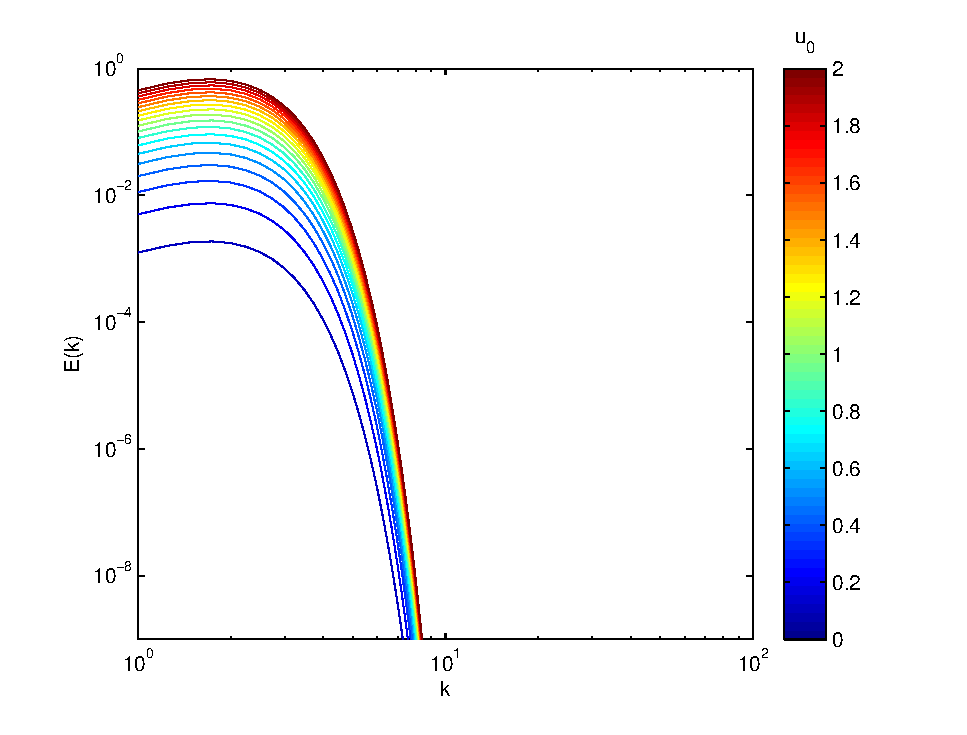
\includegraphics[width=0.48\linewidth]{Figures/eng_spr_u}
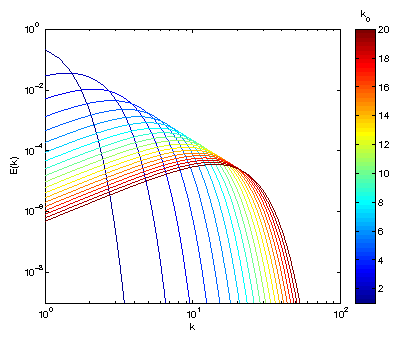
\includegraphics[width=0.48\linewidth]{Figures/eng_spr_k}
\caption{Initial energy spectra with different parameters. Left figure shows the energy spectra with fixed $k_0 = 2.4$ but varing $u_0$ from $0m/s$ to $2m/s$; right figure shows the spectra with fixed $u_0 = 0.35m/s$ and varing $k$ from $1$ to $20$.\label{fig:eng_spr}}
\end{figure}

\subsection{Initial fields of vapor mixing ratio and temperature}
Three different initial configurations of cloudy area are used to investigate the impact of cloudy area configuration. Case 1 follows that used in \citep{And04} whereby water mixing ratio is defined according to the sign of the velocity function in physical space such that
\begin{equation}
\mbox{case 1: } q_v(\mathbf{x},t=0) = 
\left\{\begin{array}{lr}
q_v^{max}, & u(\mathbf{x}) > 0\\
q_{v,e}, & u(\mathbf{x}) \le 0
\end{array}\right.\label{case1}
\end{equation}
where $q_v^{max} = 3.95 g/kg$ is the maximum amplitude of $q_v$, which exceeds $q_{v,s}$ by $2\%$, and $q_{v,e} = 0.03g/kg$ is the vapor mixing ratio of the clear air. $u(\mathbf{x})$ is the $x$ component of the fluid velocity. 

In \citep{Kumar11}, the author investigated a slab-like cloud configuration approximated with a smooth function to avoid the Gibbs phenomenon. Similarly, our Case 2 is designed to study the slab-like configuration but approximated with a simple discontinuous function given by
\begin{equation}
\mbox{case 2: } q_v(x,t=0) = 
\left\{\begin{array}{lr}
q_v^{max}, & (L-d)/2 \le x < (L+d)/2\\
q_{v,e}, & \mbox{elsewhere}
\end{array}\right.\label{case2}
\end{equation}
where the $q_v^{max}$ and $q_{v,e}$ are the same as in Case 1.
$L$ is the length of computational domain, and $d = L/2$ is the width of the cloud slab.

It is well known that entrainment-mixing processes can also occur near cloud tops, esp., for stratiform clouds \citep{Lu2011, Yum2015}. To mimic the cloud-top entrainment-mixing process, herein we add a new cloud configuration Case 3 by rotating Case 2 by $90$ degree.
\begin{equation}
\mbox{case 3: } q_v(z,t=0) = 
\left\{\begin{array}{lr}
q_v^{max}, & (L-d)/2 \le z < (L+d)/2\\
q_{v,e}, & \mbox{elsewhere}
\end{array}\right.\label{case3}
\end{equation}

The temperature field is initialized by imposing the neutral buoyancy condition such that \citep{Kumar14}
\begin{equation}
T(x,t = 0) = T_0 - 0.608T_0[q_v(x,t = 0) - q_{v0}]
\end{equation}
where the reference values are defined by the domain averages $T_0 = \langle T(t=0)\rangle_V$ and $q_{v0} = \langle q_v(t=0)\rangle_V$. This neutral buoyancy condition ensures the initial cloudy area having higher water vapor mixing ratio but lower temperature compared to the environment. Note that this procedure is only performed for the initial temperature field; later temperature field completely follow \Eq{eq:Temp} afterwards. \Fig{fig:slice_case123} compares the initial fields of  supersaturation and temperature for the three cases. The discrepancies between the initial water vapor 
and temperature fields are self-evident, allowing for examination of the impacts of the initial 
configuration of cloudy area on entrainment-mixing processes. Note that all the three initial 
configurations have the same dynamical field and initial cloud fraction of $0.5$.

\begin{figure}\centering
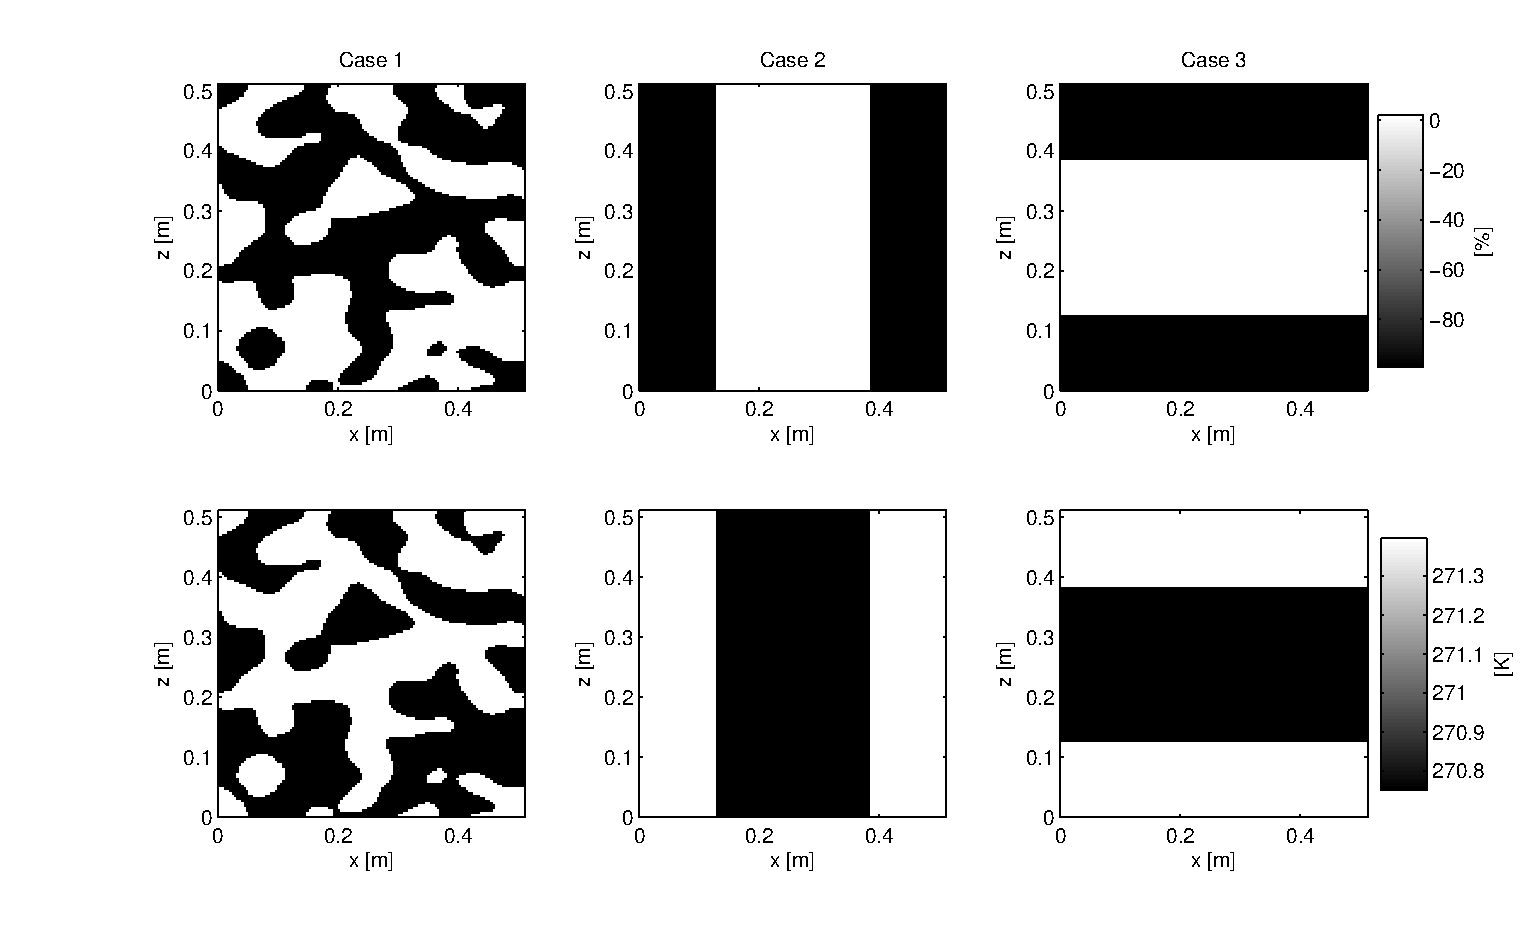
\includegraphics[width=0.9\linewidth]{Figures/init_vapor_supersat}
\caption{Cross sections of the initial supersaturation and temperature (K) field for different cases. The cloudy part occupies about half of the computational domain.\label{fig:slice_case123}}
\end{figure}

\subsection{Initial droplets}

At beginning, a total of $10^{7}$ droplets with the same radius of $15\mu m$ are randomly placed in the cloudy area according to the Poisson point process, giving a droplet number concentration of $153{cm}^{-3}$. Note that for the forced turbulence mode, the velocity field needs a few steps ($5$ seconds here) to relax to a steady state. Therefore, the droplets are released to move and change their sizes according to the physical laws after this spin-up period. For the decaying turbulence, the droplets are released at time $t = 0s$ since there is no needs to reach a steady state. The simulation is terminated when droplets completely evaporate or the field becomes nearly uniform (the standard deviation of supersaturation is less than $0.0002$). 

For convenience, \Table{tb:parameters} summarizes the key quantities and initial conditions.
\begin{table}[T]
\centering
\caption{Summary of key model parameters and initial conditions}
\label{tb:parameters}
\begin{tabular}{l c c c c c}
\hline
Quantity & Symbol & Value & Quantity & Symbol & Value\\
\hline
Grid points & $N$ & $256$ & Droplet radius & $R_{0}$ & $15\mu m$\\
Box length & $L$ & $0.512m$ & Environ supersat & $S_{e}$ & $-99\%$\\
Grid size & $a$ & $0.002m$ & Cloud supersat & $S_{c}$ & $2\%$\\
Viscosity & $\nu$ & $1.5\times10^{-5}m^{2}s^{-1}$ & Number concentration& $N_{c}$ & $153cm^{-3}$\\
Dissip rate& $\epsilon$ & $2.0\times10^{-3}m^{2}s^{-3}$ & Eddy turnover time & $\tau_{L}$ & $4.27s$\\
Dissip length& $\eta$ & $10^{-3}m$ & Evaporation time & $\tau_{evap}$ & $2.09s$\\
Dissip time& $\tau_{\eta}$ & $0.087s$ & Reaction time & $\tau_{react}$ & $4.52s$\\
\hline
\end{tabular}
\end{table}

\section{Numerical Results}\label{numerical_results}
Six numerical experiments are performed to represent six scenarios (denoted by D1, D2, D3, F1, F2, and F3) according to the combination of the two different turbulence modes (decaying vs forced) and three different initial configurations of cloudy area (Case 1, Case2, and Case 3). This section presents the results, with a focus on entrainment-mixing processes. Note that droplets with radius smaller than $1\mu m$ are excluded in the microphysical analysis. 

\subsection{Evolution of dynamical and thermodynamic fields}
\Fig{fig:therm_dynam} compares between the six simulations the temporal evolution of the domain mean, standard deviation and relative dispersion of turbulent kinetic energy (TKE, a, b, c), of temperature (d,e,f) and water vapor mixing ratio (g, h, i), and supersaturation (j, k, l). Relative dispersion is defined as the ratio of the standard deviation to the mean of the corresponding variables. As expected, the mean TKE and its standard deviation for the three forced turbulence simulations (F1, F2 and F3) remain approximately constant determined by the large scale forcing after a short relaxation from the initial time. However, it is interesting to observe a transient turbulence enhancement before gradually decaying to zero in the decaying cases, especially for D2 and D3. This transient enhancement results likely from the buoyancy effect, which is caused by the deviation of temperature and vapor mixing ratio to the reference value according to \Eq{eq:source_term}. The D3 simulation exhibits the strongest enhancement, followed by D2. But for D2 the enhancement lasts longer. The mixing in D3 is accelerated by the sedimentation effect, making it a slightly stronger and faster than D2. Note that D1 can be regarded as the intermediate stage of mixing process in D2 or D3, and therefore the buoyancy effect quickly disappear and show little enhancement in the figure.  Most of the droplets have a chance to enter the clear air and evaporate at an early stage. Evaporation process absorbs latent heat from the environment, resulting in deviation of the temperature field from the mean value. The transient enhancement can be seen more clearly from the standard deviation of temperature. The transient enhancement is weaker for the three forced simulations F1, F2 and F3 (but still stronger than that of TKE).  It is noteworthy that the behavior of transient turbulence enhancement does not appear in the field of water vapor mixing ratio, which is consistent with \citep{Kumar14}. Note that the vapor mixing ratio in the clear air is much lower than in the cloudy air. The droplets entering the clear area quickly evaporate while the droplets staying in the cloudy area continue to grow by condensation. This phase transition process reduces the difference of vapor mixing ratio between clear air and cloudy air, thus the transient growth of the deviation can hardly be observed.  The behavior of supersaturation reflects the combination of temperature and water vapor mixing ratio, as expected. The variations manifest themselves in the plots of relative dispersion.

\begin{figure}[!htbp]\centering
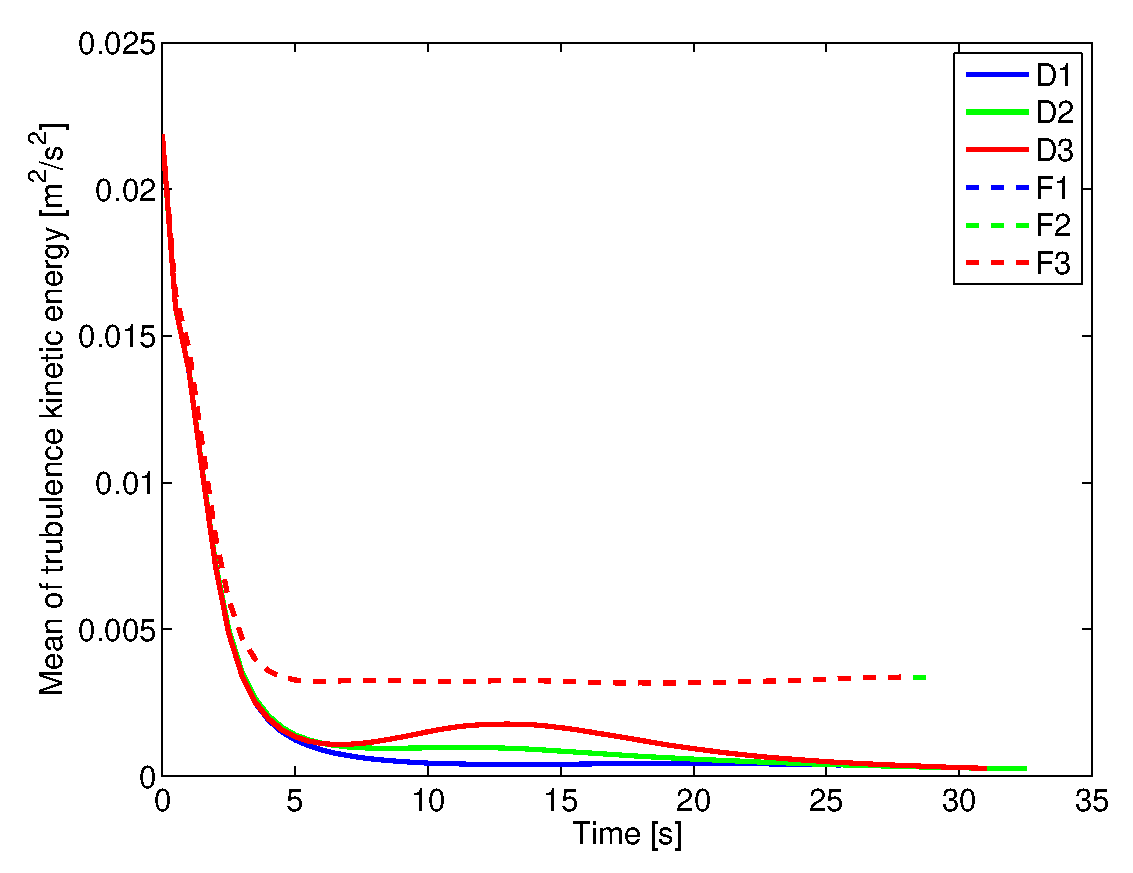
\includegraphics[width=0.3\linewidth]{Figures/mean_tke}
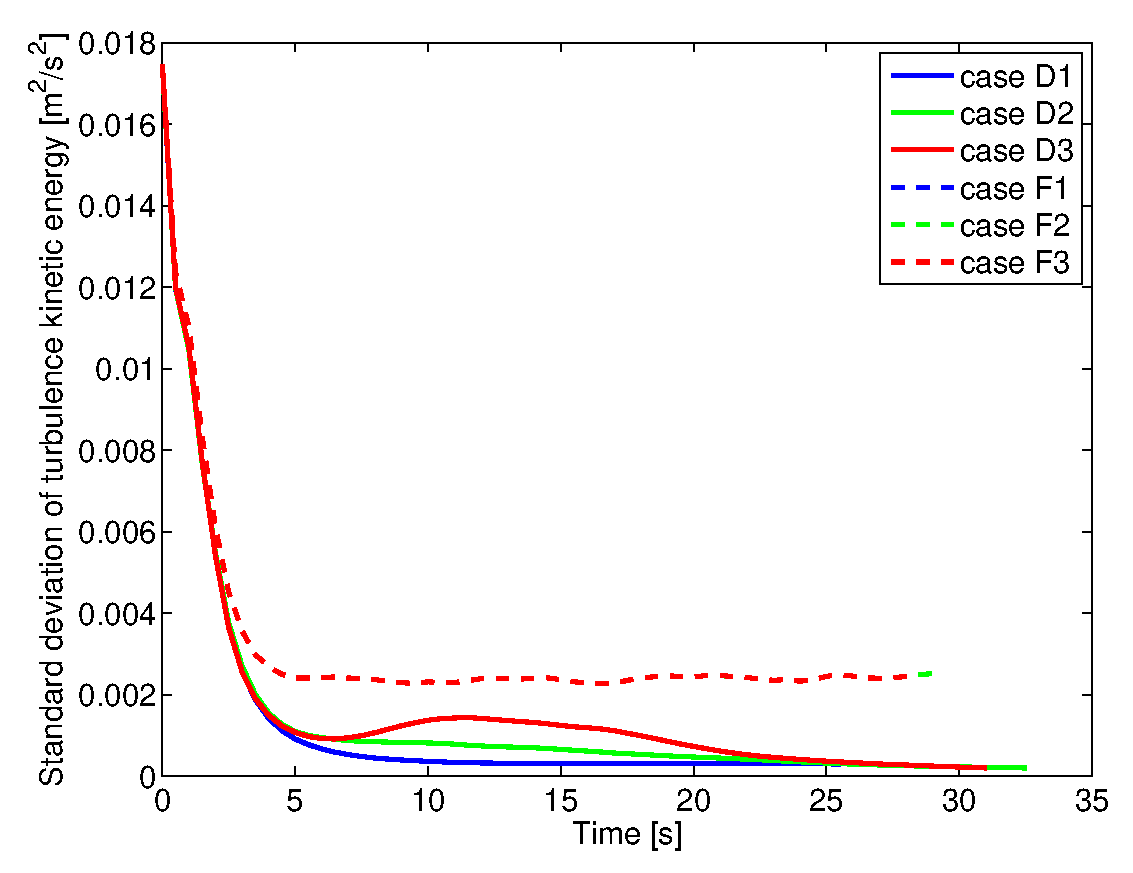
\includegraphics[width=0.3\linewidth]{Figures/std_tke}
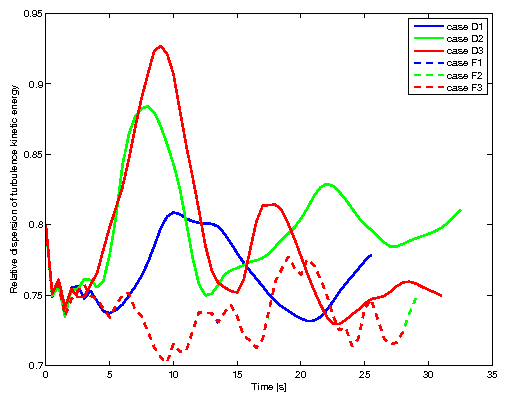
\includegraphics[width=0.3\linewidth]{Figures/dsp_tke}\\
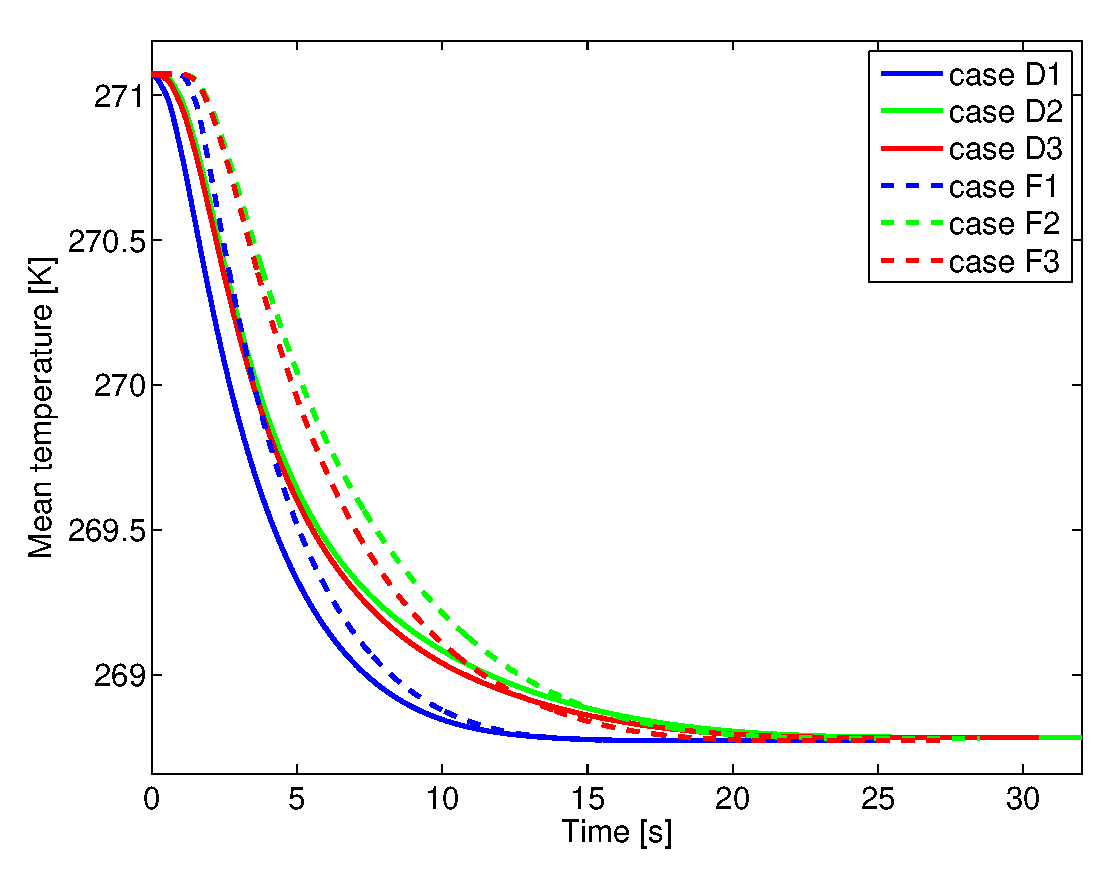
\includegraphics[width=0.3\linewidth]{Figures/mean_temp}
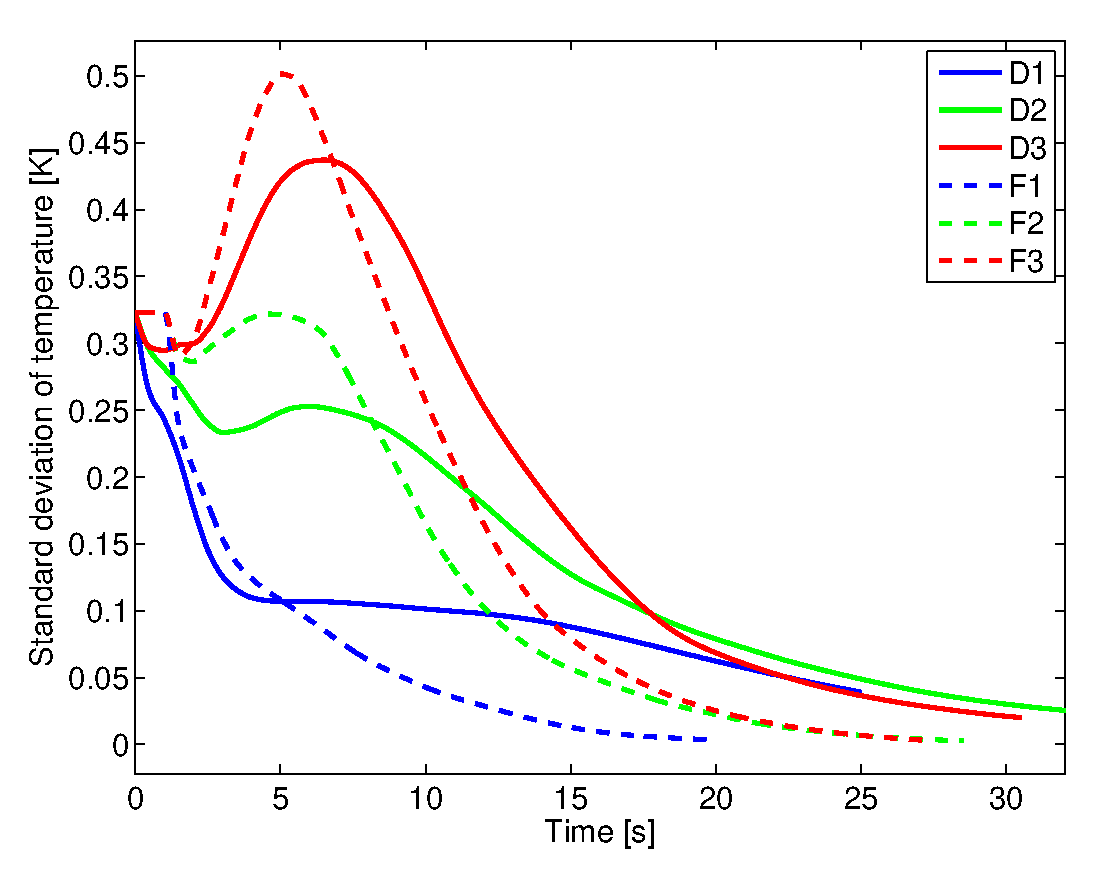
\includegraphics[width=0.3\linewidth]{Figures/std_temp}
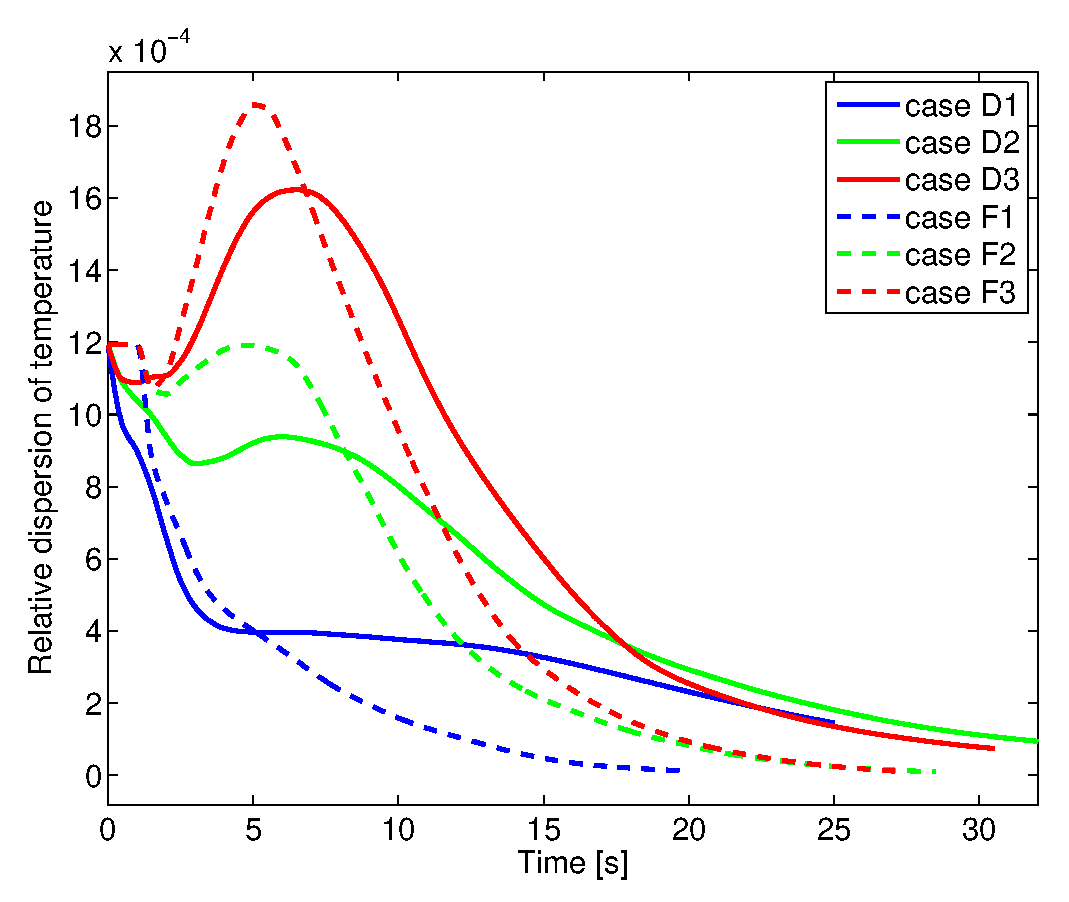
\includegraphics[width=0.3\linewidth]{Figures/dsp_temp}\\
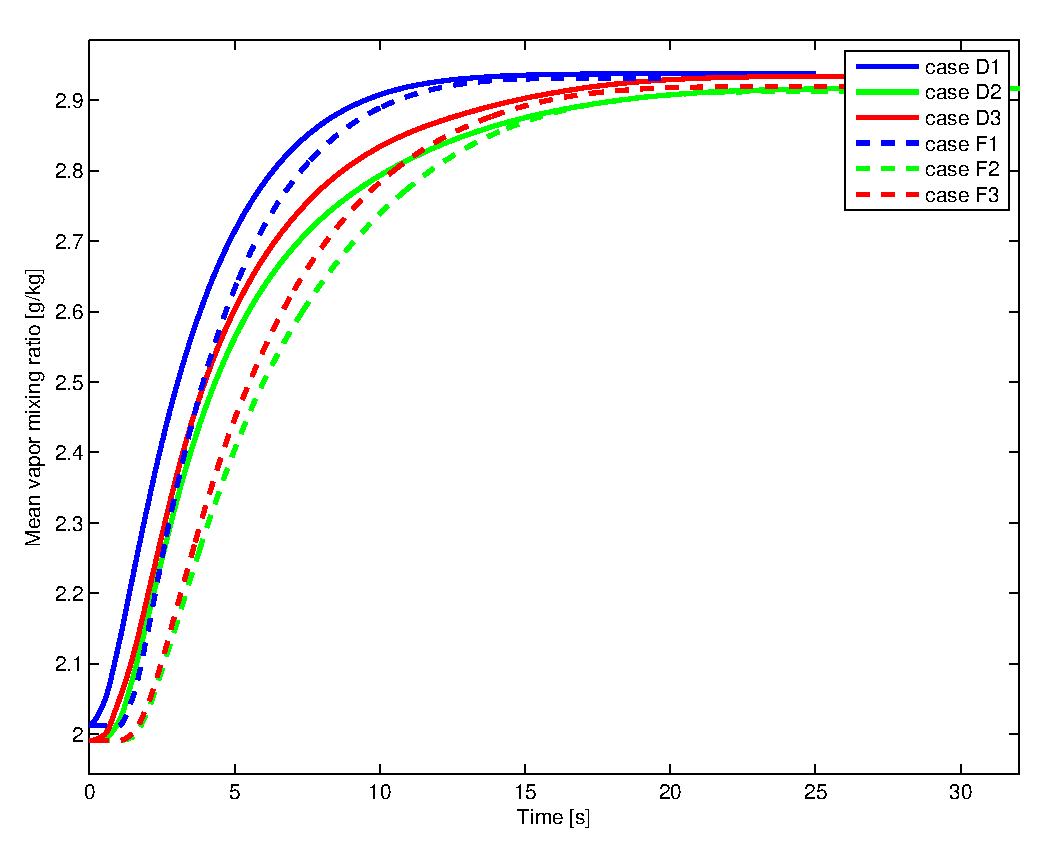
\includegraphics[width=0.3\linewidth]{Figures/mean_vapor}
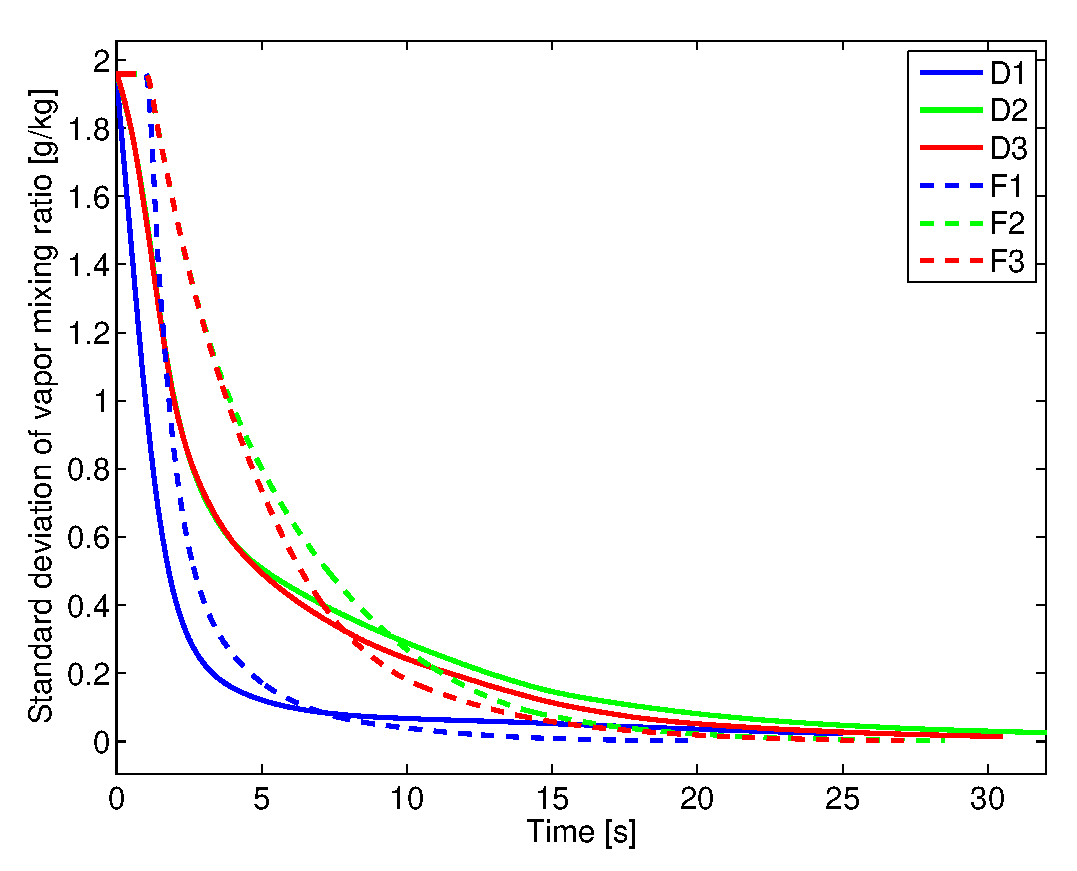
\includegraphics[width=0.3\linewidth]{Figures/std_vapor}
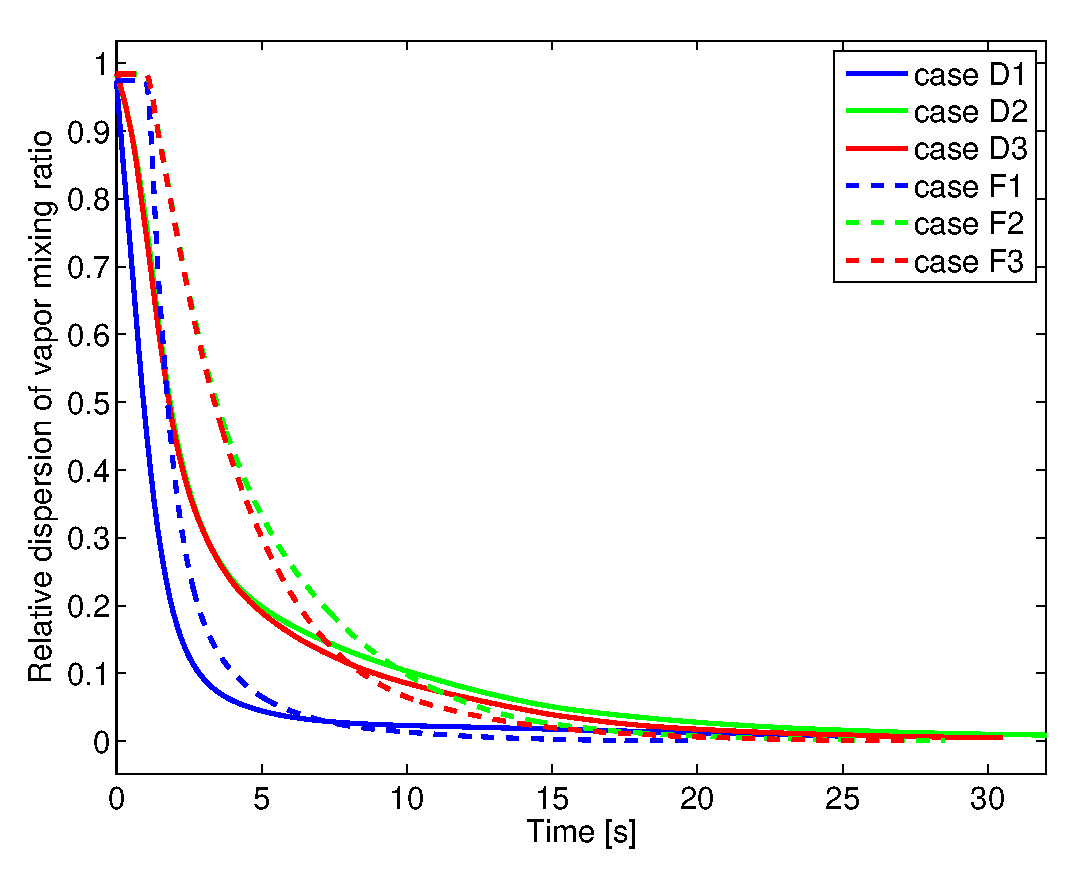
\includegraphics[width=0.3\linewidth]{Figures/dsp_vapor}\\
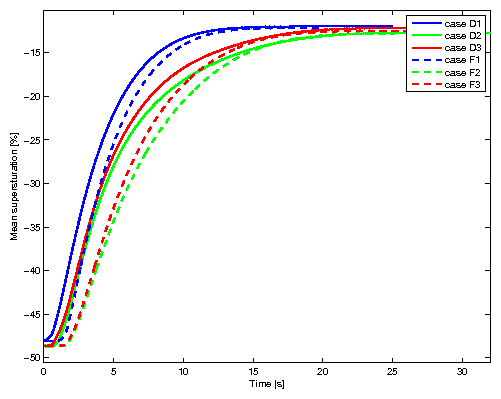
\includegraphics[width=0.3\linewidth]{Figures/mean_super}
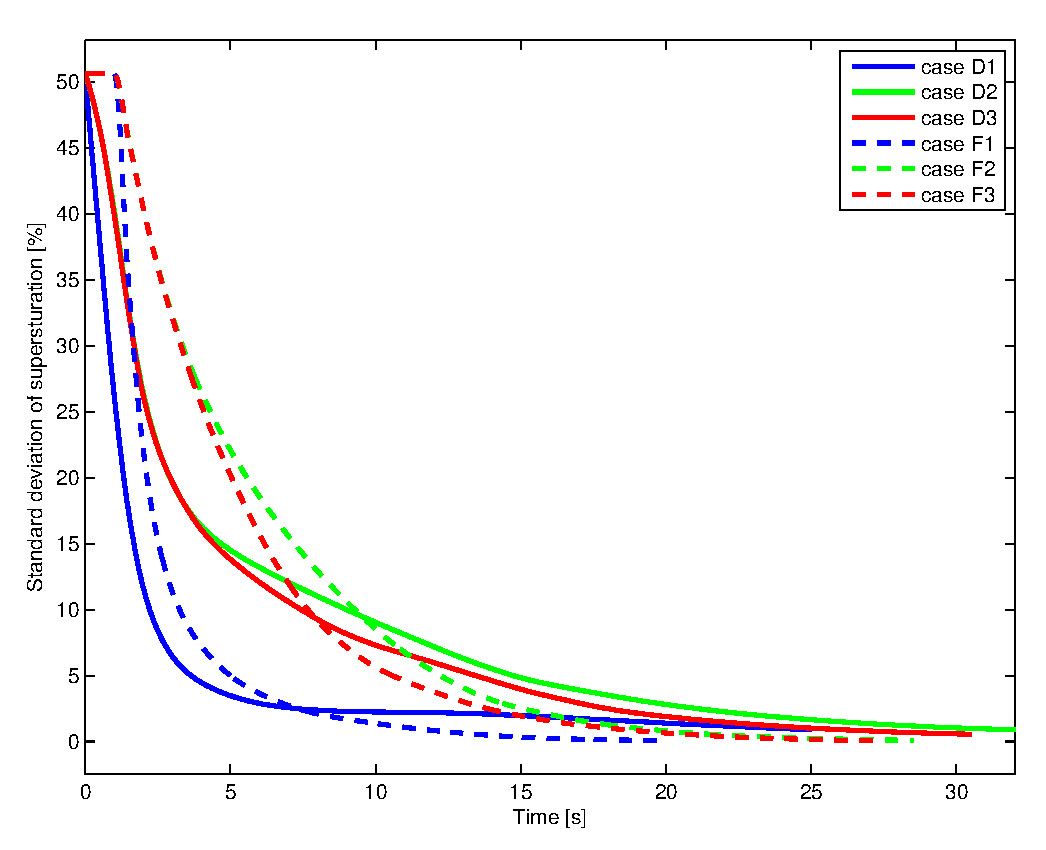
\includegraphics[width=0.3\linewidth]{Figures/std_super}
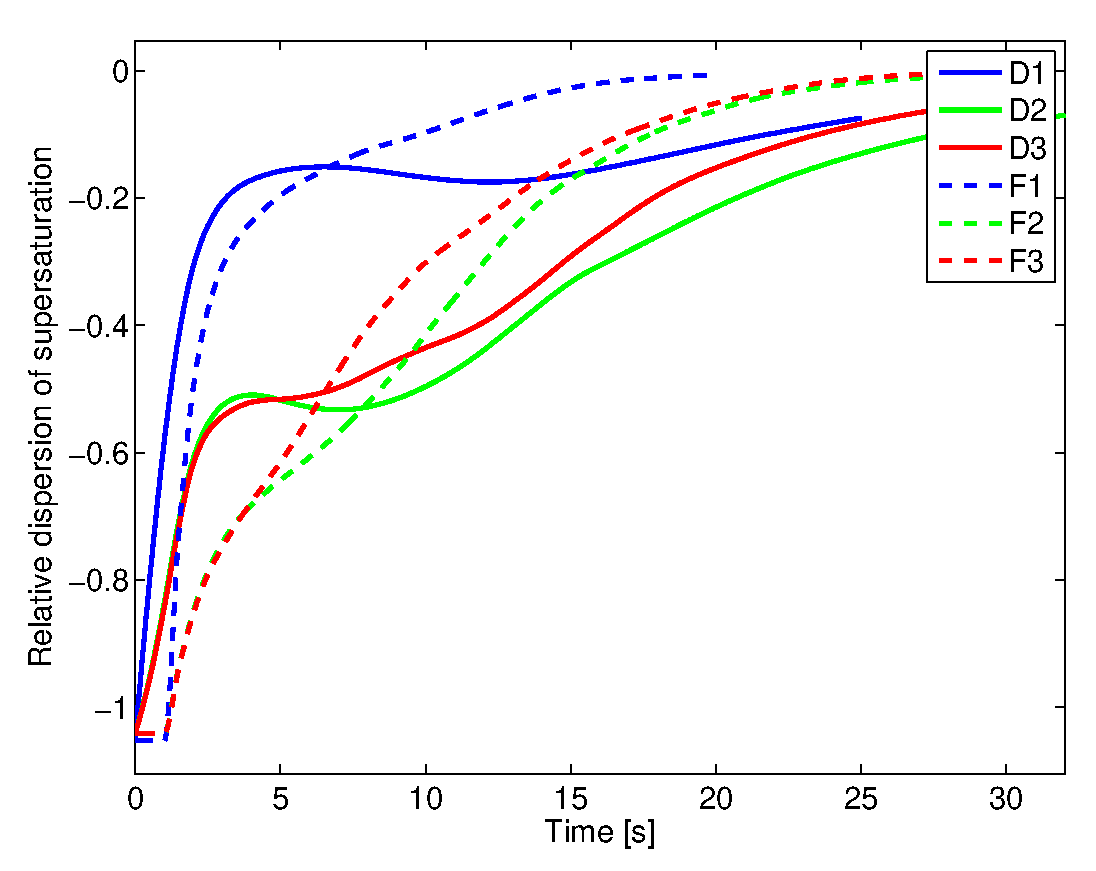
\includegraphics[width=0.3\linewidth]{Figures/dsp_super}
\caption{Temporal changes of key properties. The left, middle and right columns are the mean, standard deviation, and relative dispersion, respectively. The rows from top to bottom are turbulent kinetic energy, temperature, vapor mixing ratio and supersaturation, respectively.\label{fig:therm_dynam}}
\end{figure}

\subsection{Evolution of microphysical properties}
\Fig{fig:rad_distri} shows the temporal variation of the cloud droplet size distribution for all the six simulations. Several points are evident. First, the droplets start with a monodisperse distribution droplet radius of $15\mu m$. As the turbulent mixing between the subsaturated environment and the supersaturated cloudy air proceeds, some droplets evaporate, the size distributions gradually shift to small sizes and broadens until all droplets completely evaporate. Due to the initial configuration, the final states of all the cases contain no droplets and are in subsaturated environments. Second, the three cases in decaying turbulence (D1, D2 and D3) are quite different in their evolution of size distributions. However, the difference between the three forced turbulence cases (F1, F2 and F3) almost disappear, demonstrating that the buoyancy effect is overwhelmed by the external forcing and the differences in the decaying cases are caused by the buoyancy term in \Eq{eq:source_term}. The role of buoyancy in spectral broadening is also evident from the comparison of the corresponding simulations in modes of decaying and forced turbulence.
\begin{figure}[!htbp]\centering
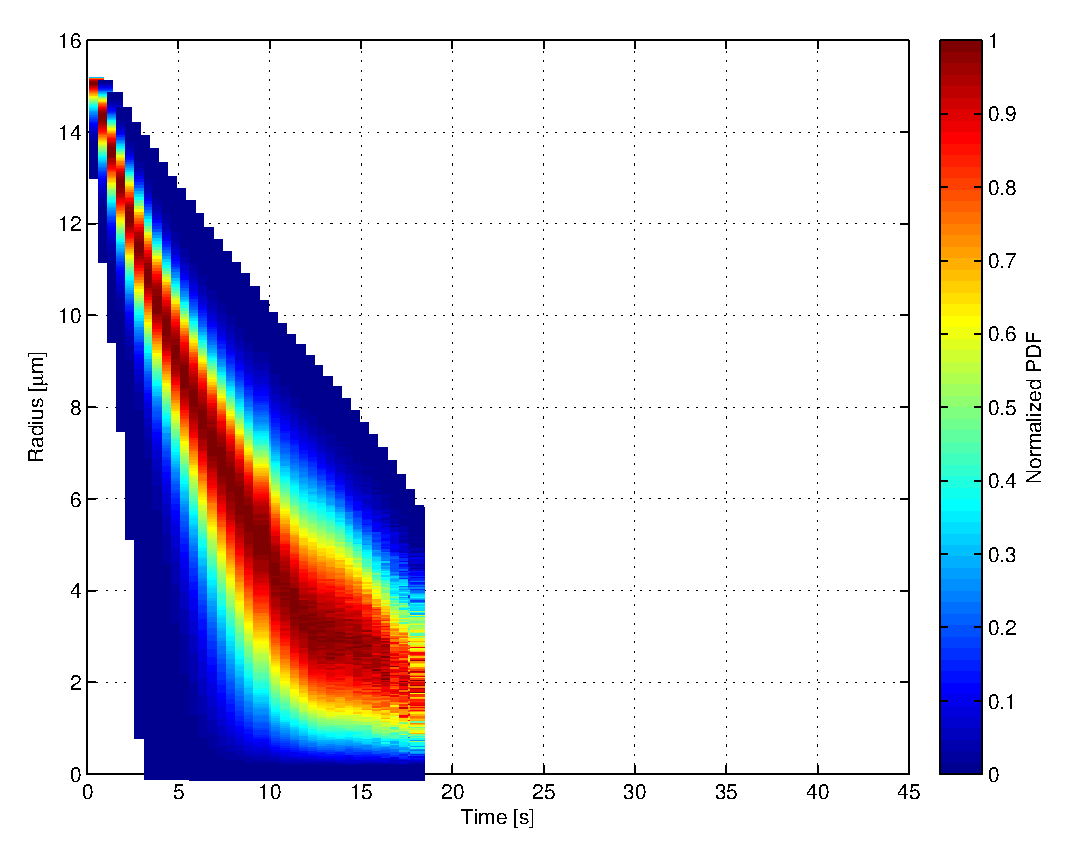
\includegraphics[width=0.48\linewidth]{Figures/pdf_radius_d1}
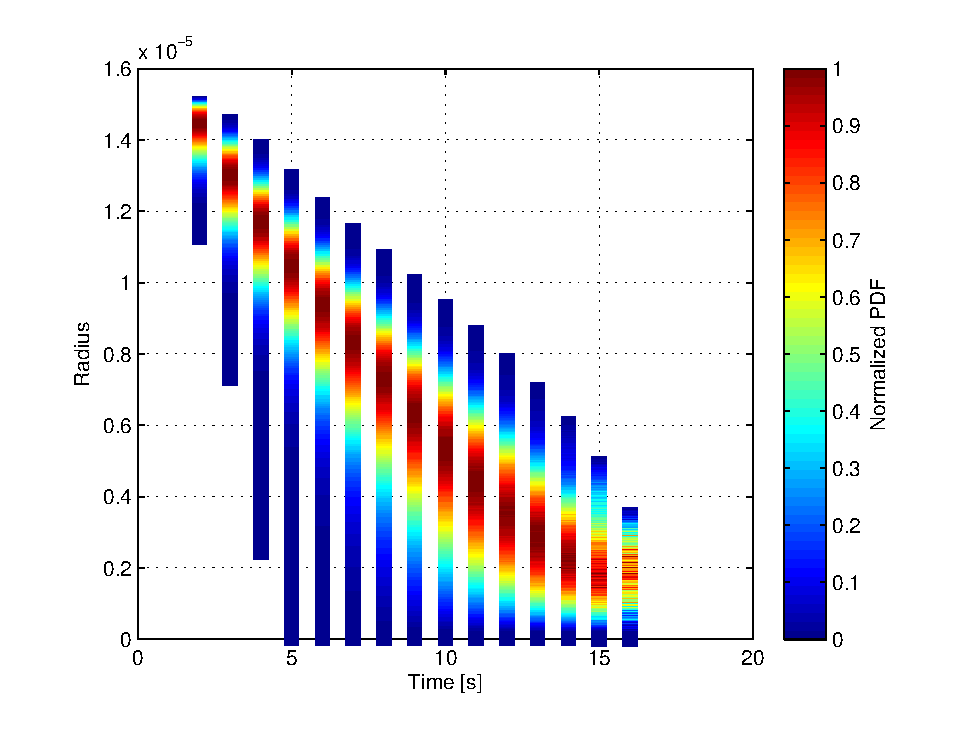
\includegraphics[width=0.48\linewidth]{Figures/pdf_radius_f1}\\
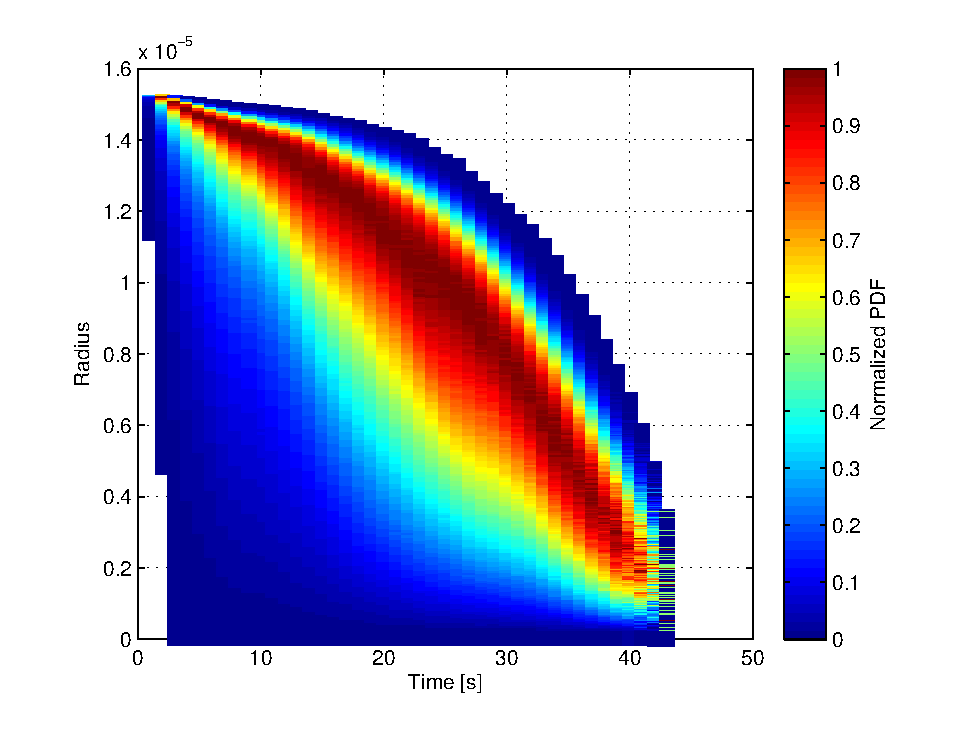
\includegraphics[width=0.48\linewidth]{Figures/pdf_radius_d2}
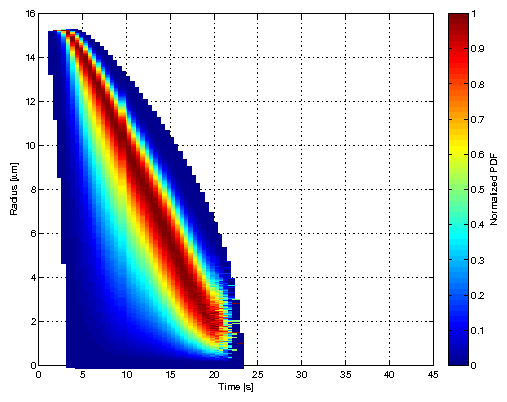
\includegraphics[width=0.48\linewidth]{Figures/pdf_radius_f2}\\
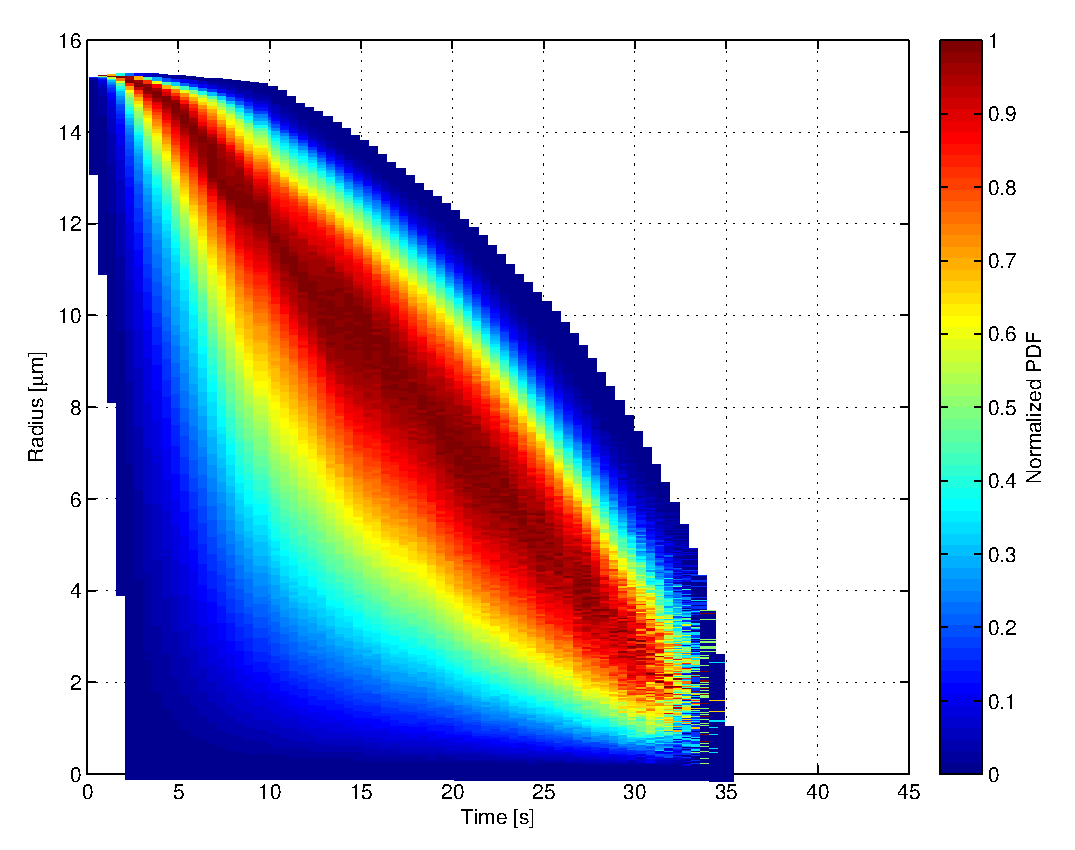
\includegraphics[width=0.48\linewidth]{Figures/pdf_radius_d3}
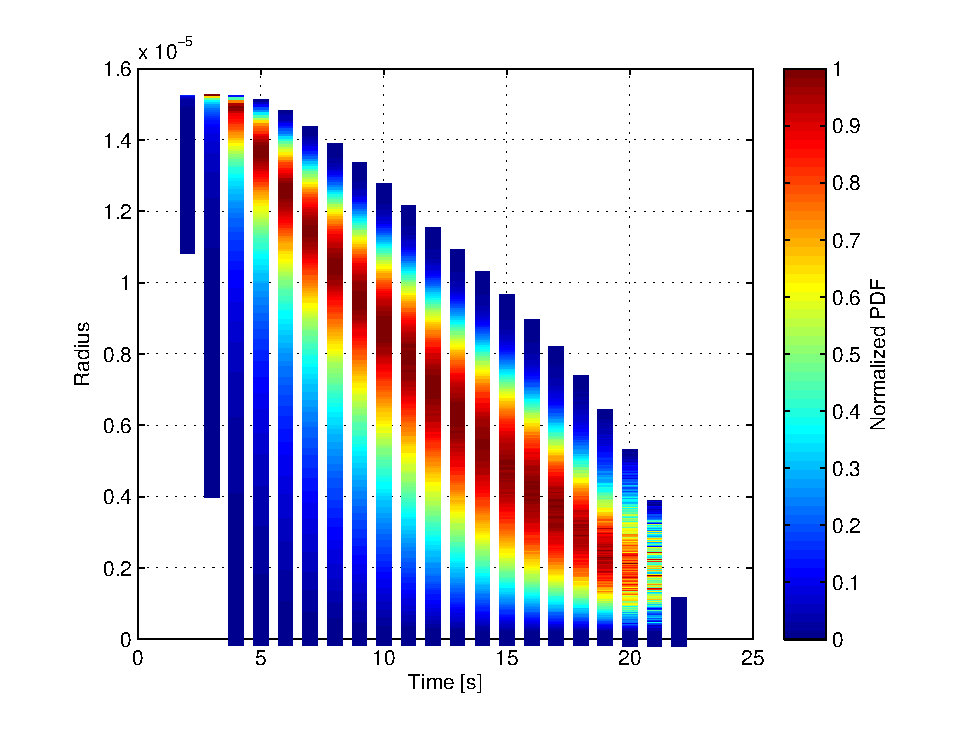
\includegraphics[width=0.48\linewidth]{Figures/pdf_radius_f3}
\caption{Evolution of droplet size distribution for decaying turbulence (left column) and forced turbulence (right column). The color denotes the droplet concentration normalized by the maximum concentration. The panels from up to bottom are Case 1, Case 2 and Case 3, respectively.} \label{fig:rad_distri}
\end{figure}

To better illustrate the impacts of different simulation scenarios, \Fig{fig:temporal_variation} shows the temporal evolution of the domain-mean liquid water content (a), droplet concentration (b), 
mean volume radius (c), mean radius (d), standard deviation (e) and relative dispersion of the cloud droplet size distribution(f). It is evident that in all the simulations, LWC and droplet concentration decrease as turbulent mixing and droplet evaporation proceed. The mean volume radius and mean radius also decreases with time because the decrease of liquid water content is stronger/faster than that of droplet concentration. It is noteworthy that in all the simulations, standard deviations first increase, peak at some time, and then decrease beyond the peak time. The occurrence of maximum standard deviation stems primarily from the combined spectral broadening related to entrainment-mixing processes and the shrinking of droplet populations due to evaporation of small droplets. Also noteworthy is that the peak standard deviations occur between $5s$ and $10s$ for all the six simulation scenarios. The coupled variations of mean radius and standard deviation result in relative dispersion peaking at a much later time compared to standard deviation. Despite the commonalities, the differences among the different scenarios are evident. Since the configuration of Case 1 is close to an already-mixed case, its number concentration and mean radius decay at a faster rate, and the standard deviation of the droplet size is lower than other cases. Case 2 and Case 3 exhibit no notable difference except for the number concentration. Since the mixing process of Case 3 is accelerated by the buoyancy effects in the vertical direction, the number concentration of Case 3 has a stronger decrease than Case 2. Comparison between the forced cases and decaying cases further shows two contrasting phases. In the first phase, the forced cases contain more liquid water content, larger number concentration and mean radius than the corresponding decaying cases, while the opposite is true in the later stage. This implies that the decaying cases initially have faster mixing and evaporation, but are later overtaken by the forced turbulence. 
  
\begin{figure}[!htbp]\centering
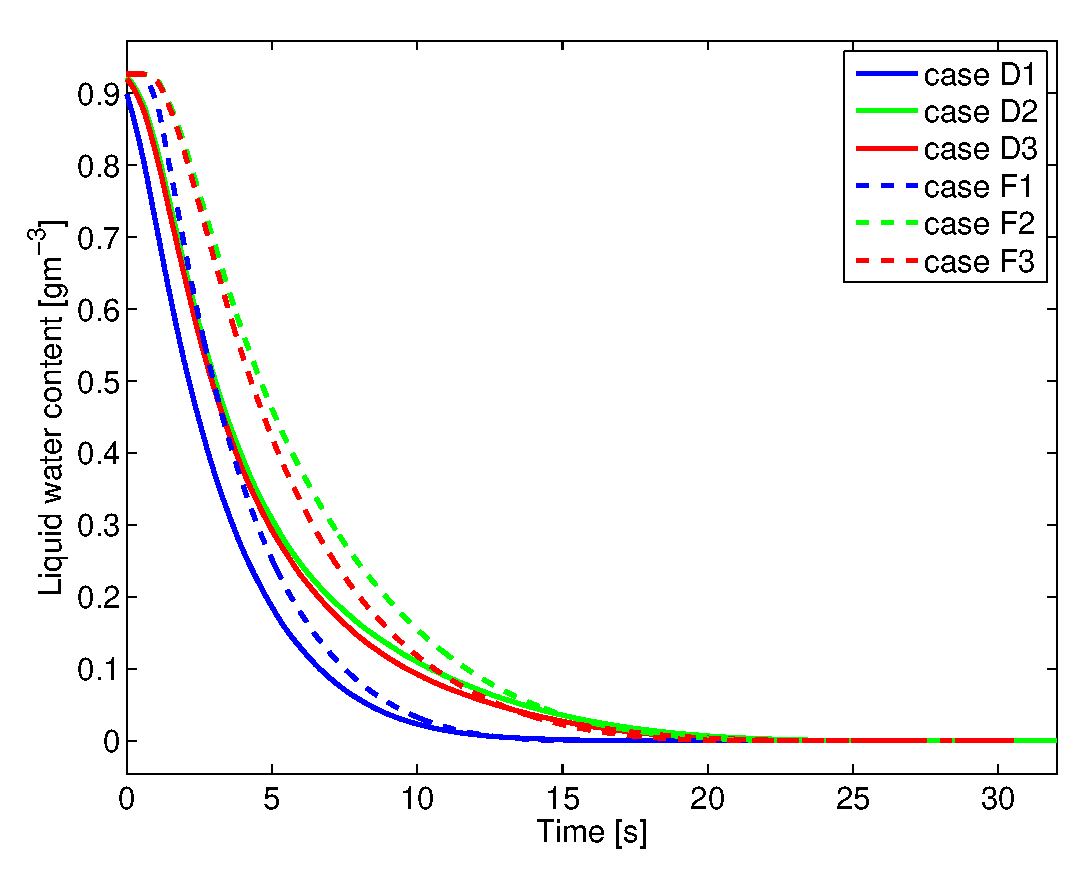
\includegraphics[width=0.48\linewidth]{Figures/lwc}
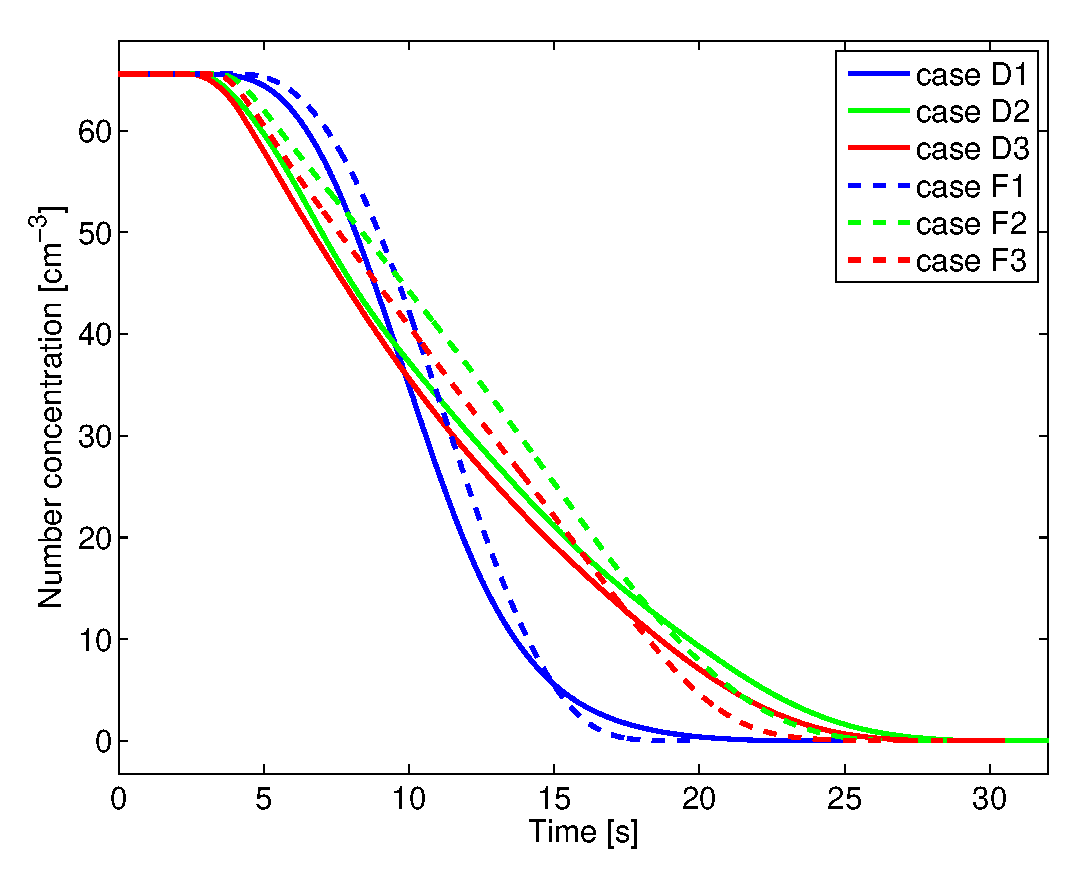
\includegraphics[width=0.48\linewidth]{Figures/num_con}\\
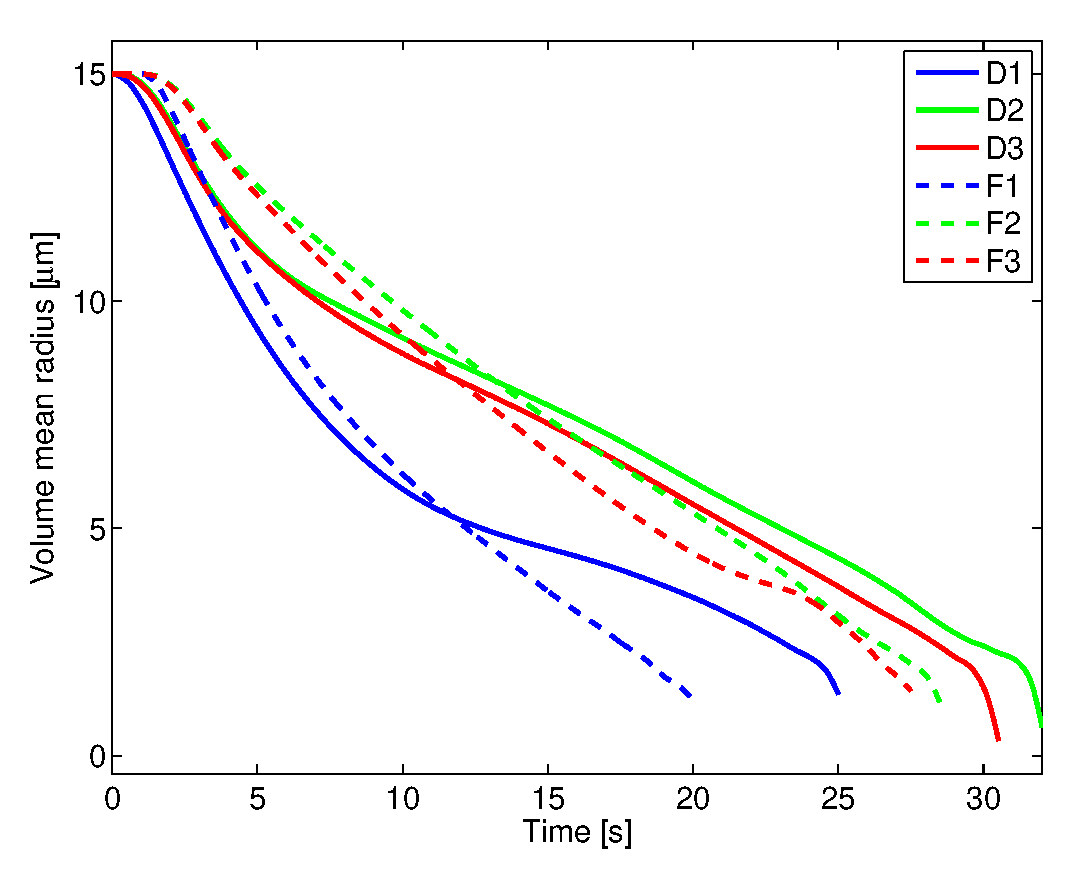
\includegraphics[width=0.48\linewidth]{Figures/vmean_radius}
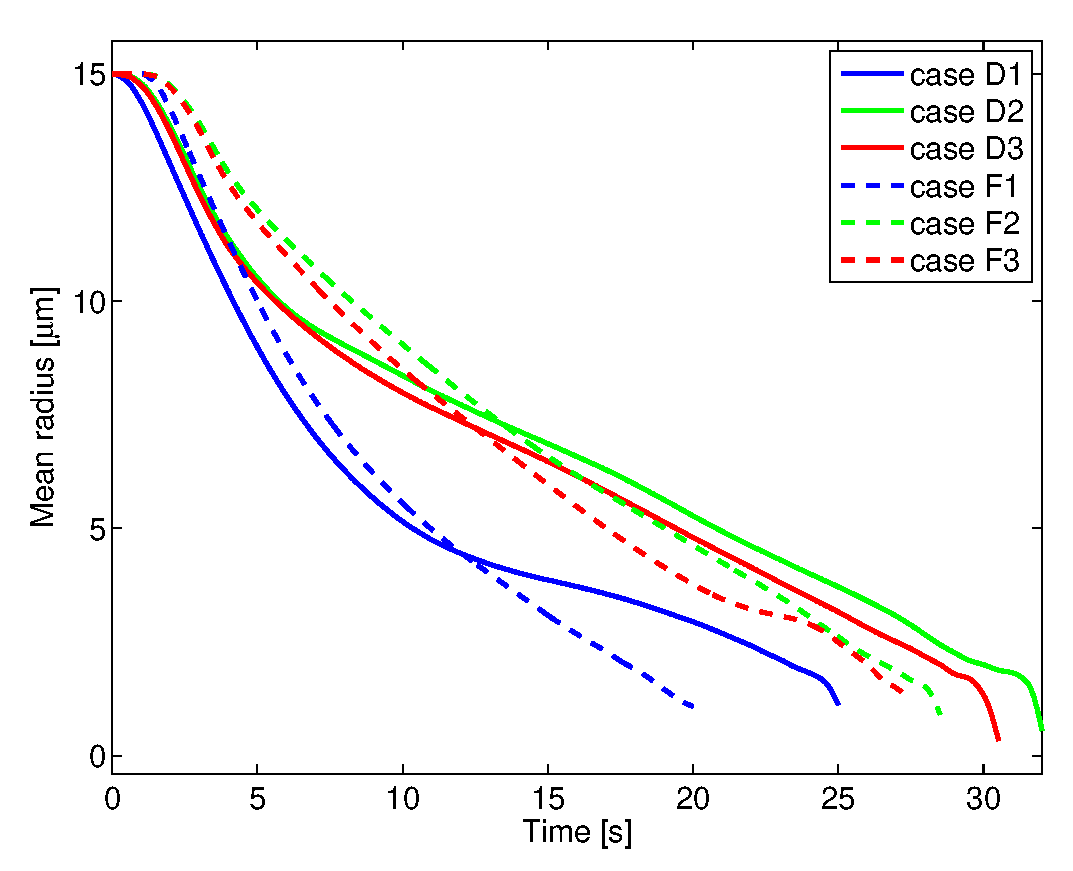
\includegraphics[width=0.48\linewidth]{Figures/mean_radius}\\
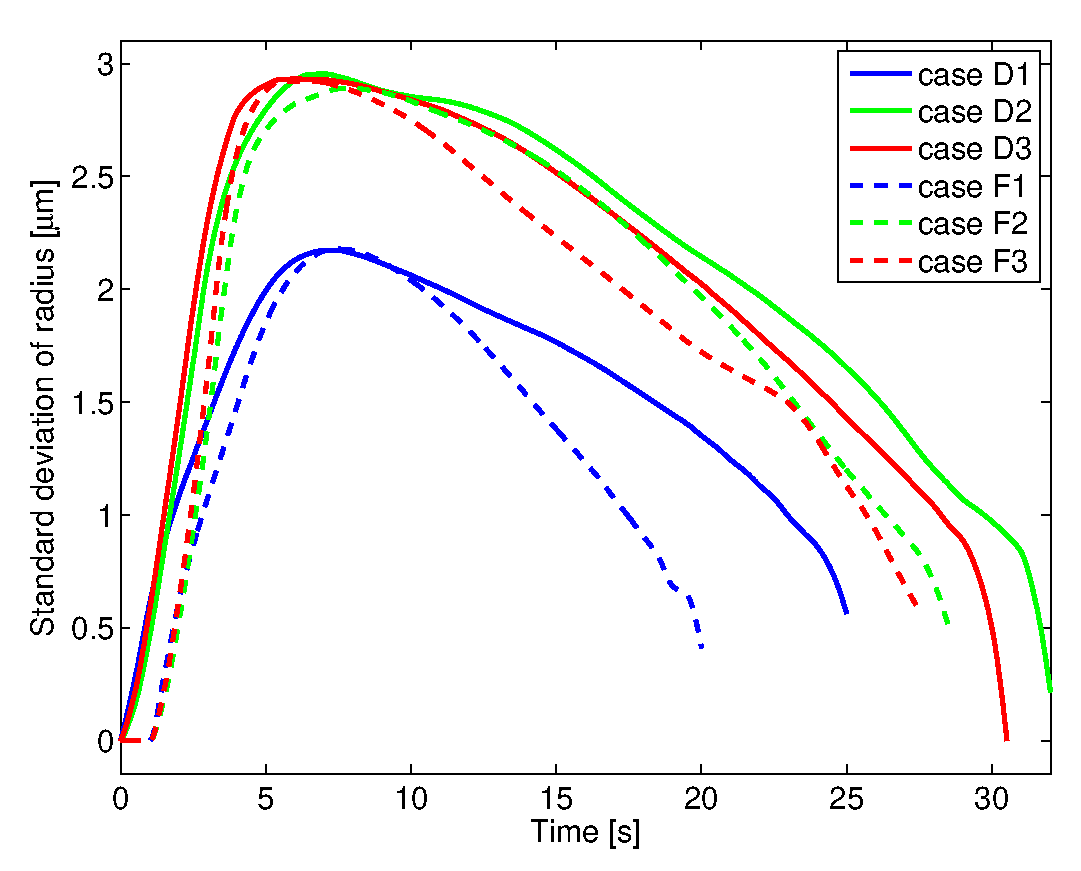
\includegraphics[width=0.48\linewidth]{Figures/std_radius}
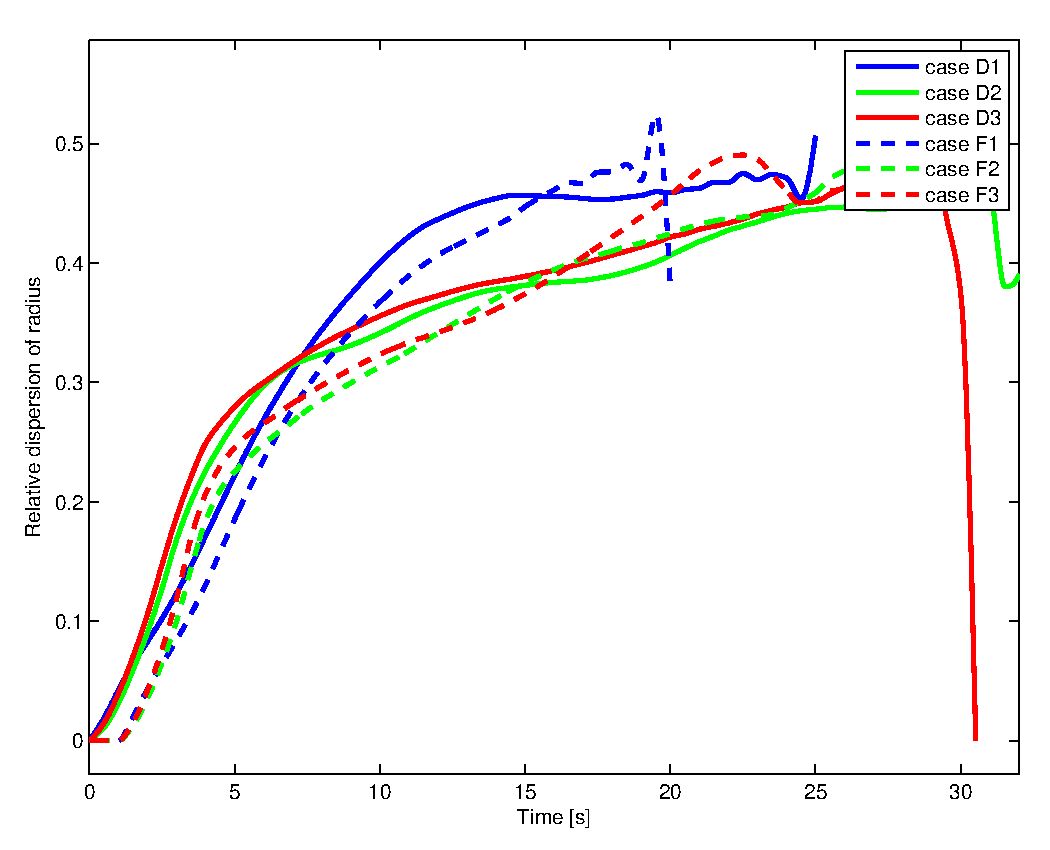
\includegraphics[width=0.48\linewidth]{Figures/dsp_radius}
\caption{Temporal evolutions of (a) droplets concentration, (b) liquid water content, (c) mean volume radius, (d) mean radius, (e) standard deviation, and (f) relative dispersion.}\label{fig:temporal_variation} 
\end{figure}

\section{Turbulent entrainment-mixing processes}\label{mixing_processes}

The impact of entrainment and subsequent cloudy-clear air mixing on the cloud droplet size distribution remains an important yet still unresolved issue in cloud physics. Although conservation of the total water and moist static energy is often adequate to determine the temperature, water vapor, and cloud water mixing ratios of the homogenized mixture of cloudy and cloud-free unsaturated air,  predicting the evolution of cloud droplet size distribution, requires additional constraints because cloud water after homogenization can be distributed over either a large number of small droplets or a small number of large droplets. The concentration and size of cloud droplets critically depend on the specific entrainment-mixing processes. Whether cloud dilution is associated with homogeneous or inhomogeneous mixing has been shown to significantly affect radiative properties of stratocumulus \citep{Chosson2007} and shallow convective clouds \citep{Grabowski2006, Slawinska2008}. However, current models ranging from large eddy simulations to climate models, lack adequate representation of the mixing mechanisms, causing deficiencies in simulated cloud microphysical properties \citep{Endo2015}. This section aims at developing physical understanding and parameterization of the entrainment-mixing processes using the DNS simulations. 

\subsection{Mixing diagram analysis}
Turbulent entrainment of dry environmental air and subsequent turbulent mixing between cloudy air and environmental air and associated droplet evaporation are likely the primary factors that affect the evolution of droplet size distributions and corresponding microphysical properties. There are two limiting entrainment-mixing mechanisms proposed in the literature. One is that the entrained air and the cloudy air are mixed evenly and all cloud droplets evaporate with the same proportion \citep{Warner1973}. This type of mixing is referred to as homogeneous mixing. The other is extreme inhomogeneous mixing, where the entrained air mixes with only some portion of cloud parcel and evaporate all droplets in this portion completely while the droplets in the rest of the cloud parcel remain intact \citep{Baker1980}. Ambient clouds often fall between the two limiting mechanisms. To characterize the effect of turbulent entrainment-mixing processes on microphysical properties, the $R_v^3-N_c$ diagram \citep{Burnet2007Observational} has been widely applied to identify the homogeneous/inhomogeneous entrainment-mixing process in observational studies and DNS simulations. \citep{And04, And06, And09} were probably the first studies that applied the mixing diagram analysis to DNS simulations with bin microphysics. \citep{Kumar14} further applied to the mixing diagram analysis to their particle-resolved DNS simulations. In addition to their model differences,  \citep{And04, And06, And09} used Case 1 initial configuration of cloudy area whereas Kumar et al. used a configuration similar to our Case 2. This section extends these pioneering studies to examine the results of all the six scenarios by use of the mixing diagram analysis.

In addition to the domain mean as examined by Andrejczuk et al, we also examine smaller averaging boxes to obtain better ideas of statistics by following \citep{Kumar14} to divide the computational domain into 64 equal-sized sample boxes. We keep tracking the volume mean radius and number concentration in each sample box and at each time step. \Fig{fig:mixing_diagram} shows the mixing diagrams for the six scenarios. The solid green dot represents the value sampled in each sample box at each time step; the red curve denotes the DNS domain average, with arrows indicating the direction of temporal evolution. The corresponding homogeneous mixing line (black dot) and extreme inhomogeneous mixing line (black solid) are plotted in the diagram as references. Note that in the top panel, the mixing diagrams for D1 and F1 do not start from the $(1,1)$ point since the initial droplets in a sample box have already been diluted and their number concentration are thus less than the adiabatic value. As pointed out by \citep{And04}, this configuration excludes the initial dilution process and can only be used to simulate the mixing process after dilution. The droplet number concentration remains nearly unchanged as the droplet size decreases until some time has elapsed, suggesting an extreme homogeneous mixing. The difference is not obvious between forced turbulence and decaying turbulence, except for a wider range of variability in the shape of the mixing trajectories for the decaying turbulence D1, since the forced turbulence will foster the mixing process, resulting in similar states in different sample boxes. 

The middle panel shows the mixing diagrams for case D2 and F2. These cases have virtually the same configurations with \citep{Kumar14}, except that a sharp initial profile of vapor mixing ratio is used in our simulation. The phenomenon of inhomogeneous offset described by \citep{Kumar14} can also be observed in the figures: the mixing trajectories tend to shift to smaller values of $N_c/N_{c,a}$. This inhomogeneous offset is due to the initial dilution process, in which the droplet number concentration in the sample boxes is diluted while the droplet mean radius in the sample box doesn't change much. As turbulent mixing proceeds, the turbulent time scale in the decaying case continues to increase while the time scale for the forced turbulence remains unchanged. Therefore, the inhomogeneous mixing is more likely to occur in D2, leading to a slightly stronger deviation from the homogeneous mixing line.  A similar conclusion can be obtained in the bottom panel for case D3 and F3. 

The mixing diagrams for case D3 and F3 are displayed in the bottom panel. Case 3 resembles most properties of Case 1 and Case 2, except that its points are more scattered than other cases. This phenomenon is likely due to the sedimentation effect, which enhances the droplets motion in the vertical direction. Since the initial cloudy area in Case 3 is vertically sandwiched between two clear air regions, the cloud droplets moving up and down can easily enter a different environment (clear region) in the early stage, and therefore it increases the variability of the scatter plots.

Also noteworthy is that the difference between the mixing diagrams lies primarily in the cloudy area configurations, esp., Case 1 vs. Case 2 or Case 3, instead of lying in whether or not the turbulence is forced or freely decaying as shown \Fig{fig:rad_distri} for the temporal evolutions of droplet size distribution.  This result suggests the potential for a unified parameterization of different mixing mechanisms detailed next.

\begin{figure}[!htbp]\centering
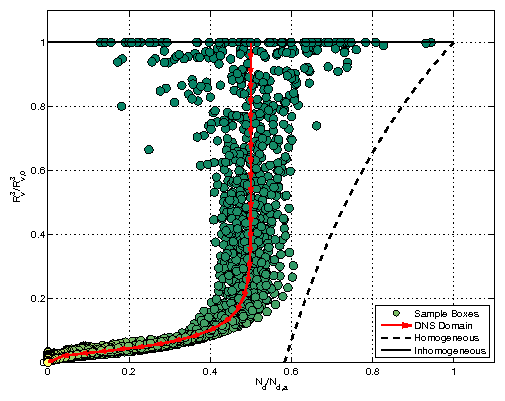
\includegraphics[width=0.4\linewidth]{Figures/mixing_cased1}
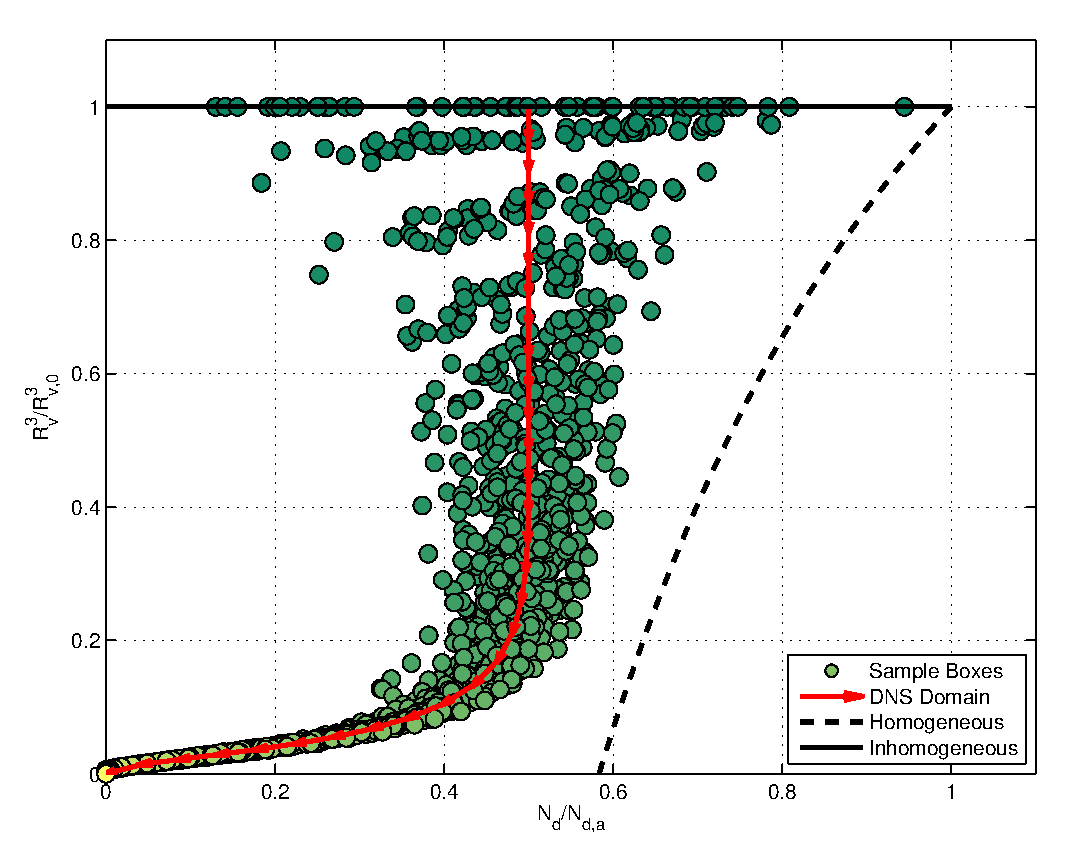
\includegraphics[width=0.4\linewidth]{Figures/mixing_casef1}
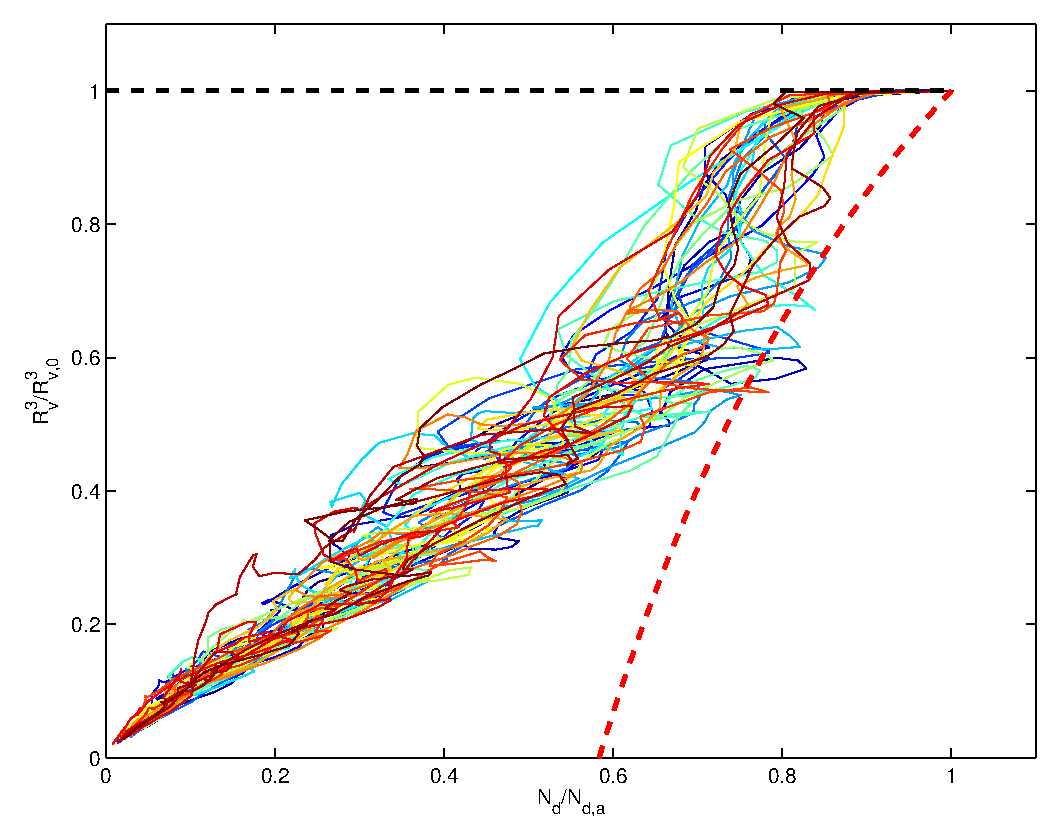
\includegraphics[width=0.4\linewidth]{Figures/mixing_cased2}
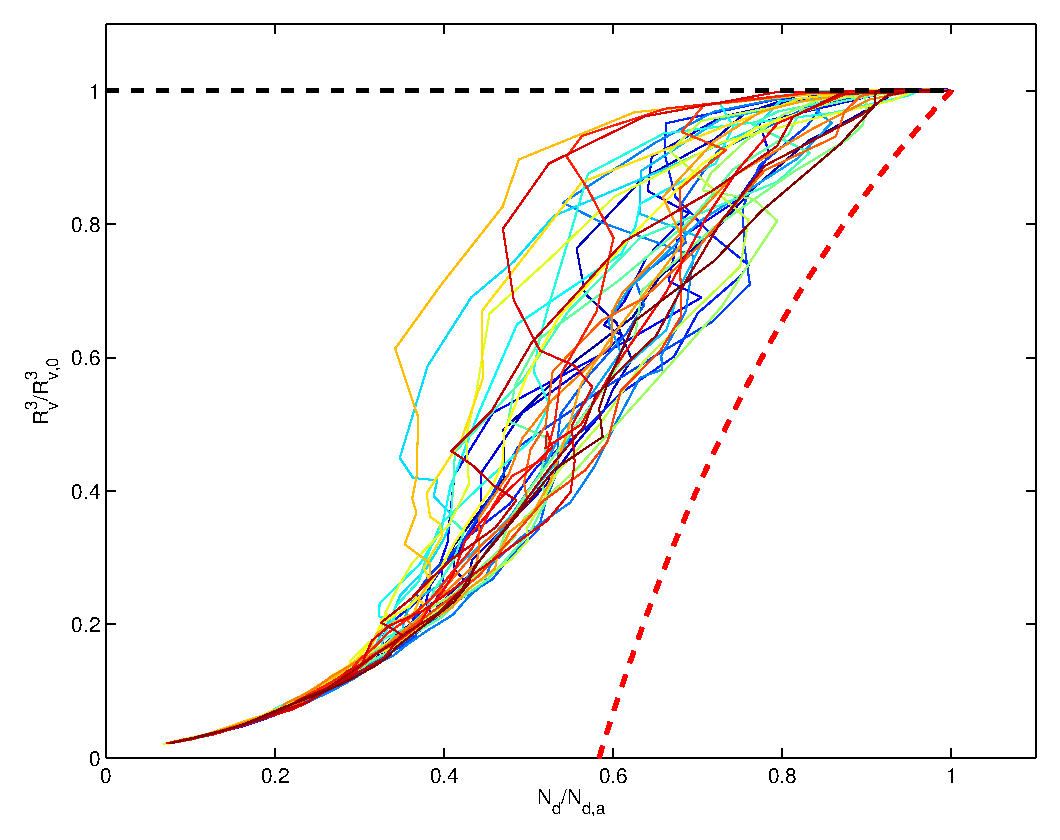
\includegraphics[width=0.4\linewidth]{Figures/mixing_casef2}
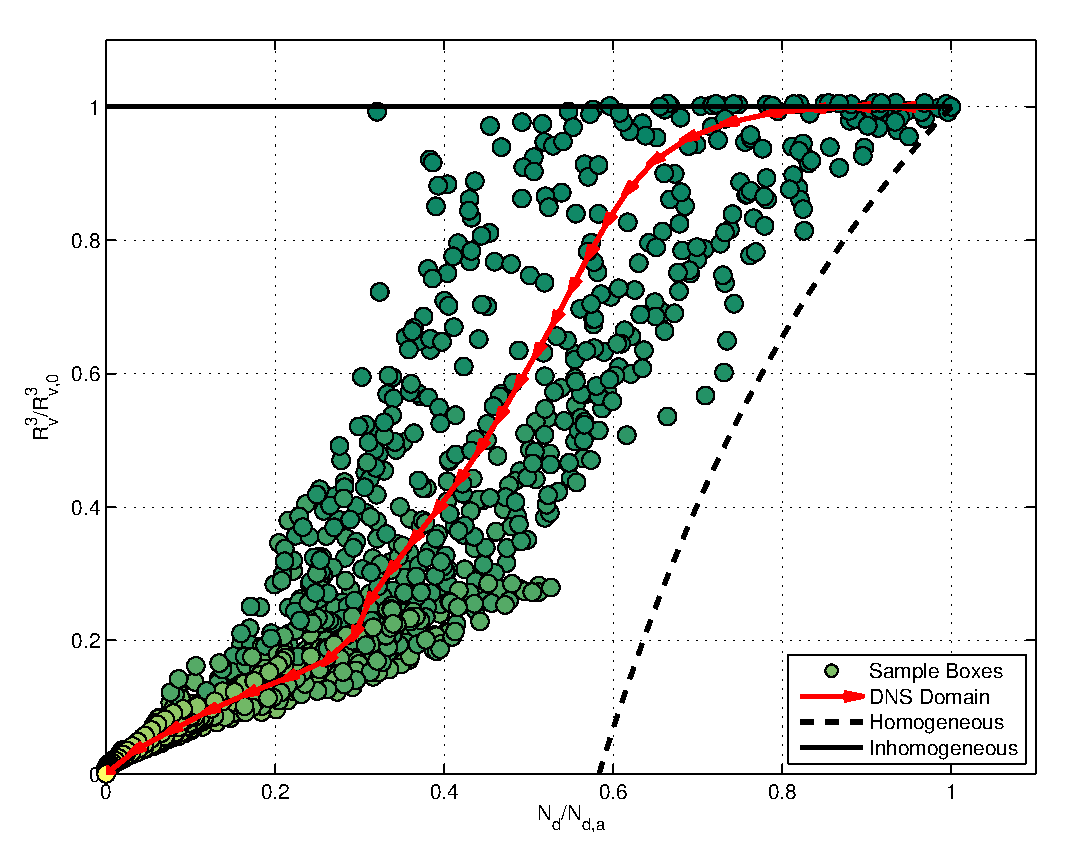
\includegraphics[width=0.4\linewidth]{Figures/mixing_cased3}
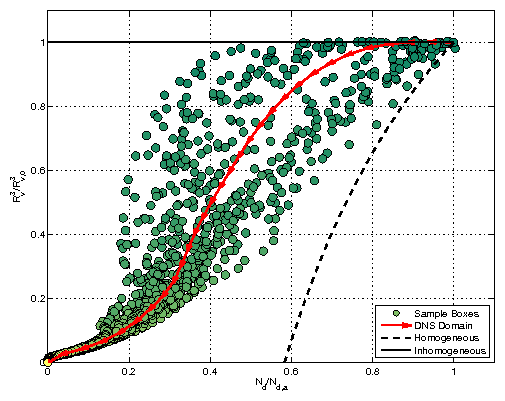
\includegraphics[width=0.4\linewidth]{Figures/mixing_casef3}
\caption{Microphysical mixing diagram for scenario D1, D2, D3, F1, F2 and F3. The green
circles represent the results for different sample boxes and the red triangles represent the mean over the entire domain, with arrow indicating the direction of time. The solid and dashed black lines denote the extreme inhomogeneous and homogeneous mixing, respectively. Only the boxes with non-zero droplets at the initial time are considered.}
\label{fig:mixing_diagram}
\end{figure}

\subsection{Analysis of microphysical measures for mixing mechanisms}
Since the real entrainment-mixing process can fall anywhere between the two limiting mixing mechanisms, it is desirable to define some measure that can cover all the possible mixing mechanisms. We generically called such a measure as homogeneous mixing degree since a larger homogeneous mixing degree indicates that the mixing process is closer to the limiting homogeneous mixing process. Based on the fact that the horizontal line in the $R_v^3−-N_c$ mixing diagram corresponds to the extremely inhomogeneous mixing whereas the vertical line implies extremely homogeneous mixing \citep{And09, Lu2013}, the homogeneous mixing degree can be quantified by the instantaneous slope of the trajectories in the mixing diagram, and is calculated using backward differencing in time: 
\begin{equation}
\psi_1 = \frac{R_{v,j}^3/R_{v,a}^3 - R_{v,j-1}^3/R_{v,a}^3}{N_{j}/N_a - N_{j-1}/N_a}
\label{phi1}
\end{equation}
where $R_v$ is the mean volume radius; $N$ is the number concentration; the subscript ``$a$'' denotes the adiabatic value of the droplet population in the initial cloudy region. Note that $\psi_1$ is in fact the inverse of the parameter defined by \citep{And09} such that a larger value of $\psi_1$ indicates a higher degree of homogeneous mixing, in line better with intuition and the other microphysical measures discussed below. It can be readily shown that $\psi_1$ equals to $0$ for the extremely inhomogeneous mixing, but approach $\infty$ as the mixing process approaches homogeneous mixing. A shortcoming of this measure lies in that it is not explicitly constrained by the limiting homogeneous and/or inhomogeneous mixing types. To overcome this deficiency, \citep{Lu2013, Lu2014} introduced more measures of homogeneous mixing degree. These measures are based on the mixing of adiabatic cloudy air and clear air, and slightly modified here to consider the instantaneous homogeneous mixing degree between two adjacent 
temporal states in time $t_j$ and $t_{j-1}$, such that
  
\begin{subequations}
\begin{equation}
\psi_2 = \frac{\beta}{\pi/2}
\label{phi2}
\end{equation}

\begin{equation}
\beta = \tan^{-1}(\frac{R_{v,j}^3/R_{v,j-1}^3 - 1}{N_j/N_{j-1} - N_H/N_{j-1}}) \text{ for } N_j < N_H, \text{ or}
\end{equation}

\begin{equation}
\beta = \pi + \tan^{-1}(\frac{R_{v,j}^3/R_{v,j-1}^3 - 1}{N_j/N_{j-1} - N_H/N_{j-1}})  \text{ for } N_j \geq N_H
\end{equation}
\end{subequations}

\begin{equation}
\psi_3 = 0.5(\frac{N_j-N_{I}}{N_H-N_I} + \frac{R_{v,j}^3-R_{v,j-1}^3}{R_{v,H}^3 - R_{v,j-1}^3})
\label{phi3}
\end{equation}

\begin{equation}
\psi_4 = \frac{\ln R_{v,j}^3 - \ln R_{v,j-1}^3}{\ln R_{v,H}^3 - \ln R_{v,j-1}^3}
\label{phi4}
\end{equation}

\begin{equation}
\psi_5 = \frac{1 - R_{v,j}^3/R_{v,j-1}^3}{1 - LWC_{j}N_{j-1}/(N_H LWC_{j-1})}
\label{phi5}
\end{equation}

where all the variables are calculated from a sample box; $LWC$ is the liquid water content; the subscript ``$j$'' means the value is calculated from the $j$-th dataset at time $t_j$. The subscripts $I$ and $H$ indicate that the values are calculated based on the assumption of inhomogeneous and homogeneous mixing, respectively. Briefly,
\begin{equation}
N_H = \chi N_j + (1 - \chi) Ne_j
\end{equation}

\begin{equation}
R_{v,H}^3 = \frac{N_jR_{v,j}^3}{N_H},
\end{equation}

\begin{equation}
N_I = \frac{R_{v,j}^3}{R_{v,j-1}^3}N_j.
\end{equation}

The mixing fraction $\chi$ is computed according to the mass conservation of total water between state $j$ and $j-1$:
\begin{equation}
\chi(q^{j-1}_{vc} + q^{j-1}_{lc}) + (1-\chi)(q^{j-1}_{ve} + q^{j-1}_{le}) = q^{j}_{lc} + q^{j}_{vc}
\label{eq:mixing_frac}
\end{equation}
where the subscripts $c$ and $e$ stand for the mean 
value of a sample box and its environmental air; $l$ and $v$ stand for the liquid 
water and water vapor. The environmental air is chosen as the mean of the $4$ 
grids extended from the original sample box; the subscript $j$ indicates the state of the $j$-th dataset 
collected at time $t_j$. Note that \Eq{eq:mixing_frac} considers the fact that the cloudy air may have 
been diluted and the environmental air may contain droplets.

\Fig{phi_compare} compares the five measures of microphysical homogeneous mixing degree, where each dot represents an 
instantaneous domain-mean and the different color denotes the six different scenarios.
Evidently, $\psi_3$, $\psi_4$ and $\psi_5$ are virtually equivalent, with most points failing along the perfect line. The relationship between $\psi_2$ and $\psi_3$ is tight until both are larger than $1$. Despite being still largely positively correlated, the association between $\psi_1$ and $\psi_3$ is weak. 

\begin{figure}[!htbp]\centering
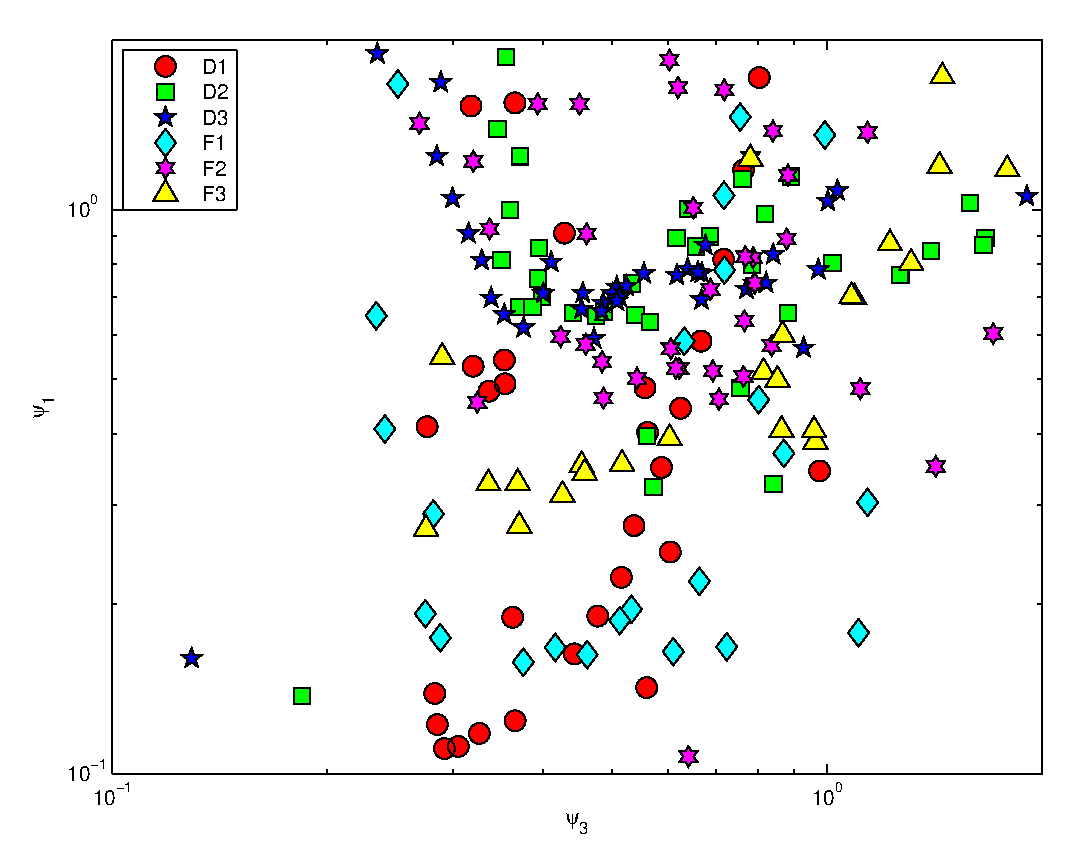
\includegraphics[width=0.45\linewidth]{Figures/phi3_phi1}
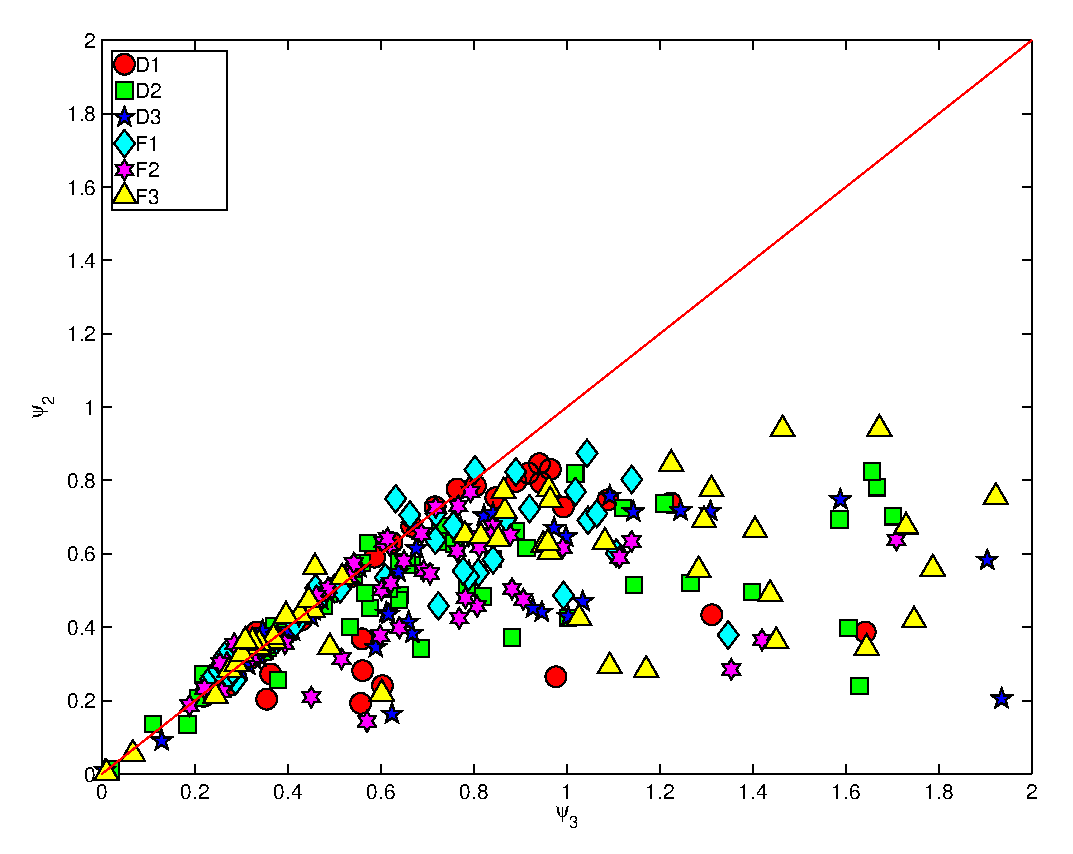
\includegraphics[width=0.45\linewidth]{Figures/phi3_phi2}\\
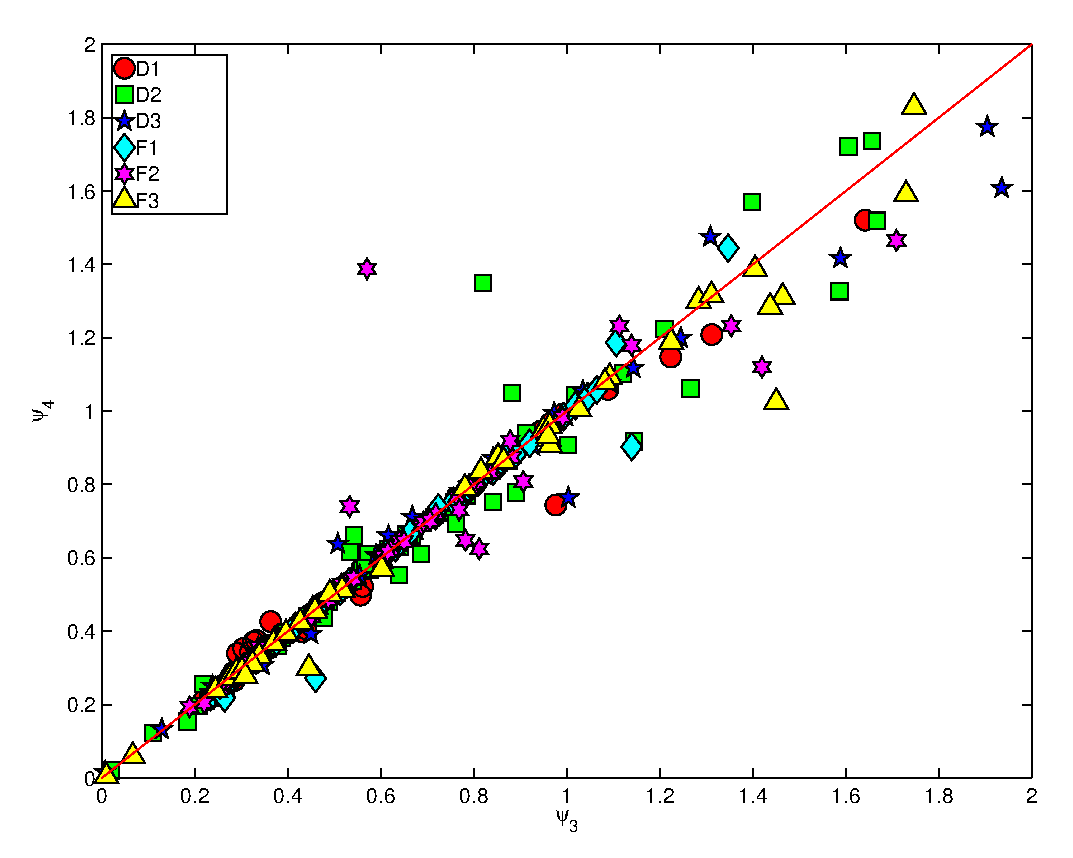
\includegraphics[width=0.45\linewidth]{Figures/phi3_phi4}
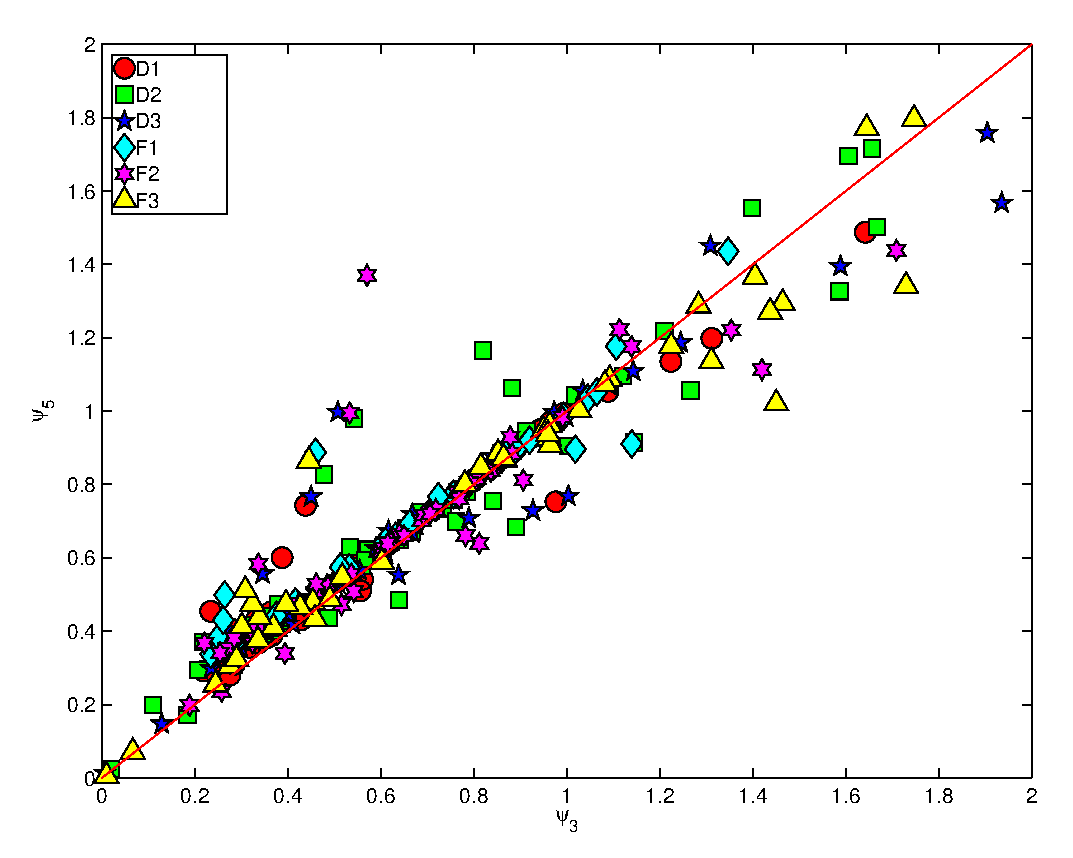
\includegraphics[width=0.45\linewidth]{Figures/phi3_phi5}
\caption{Comparison between the five measures of microphysical homogeneous mixing degree. Each dot represents an instantaneous domain-mean; different color denotes the six different scenarios.\label{phi_compare}}
\end{figure}

\subsection{Analysis of dynamical measures for mixing mechanisms}
The entrainment-mixing process has been dynamically characterized with the Damk{\"o}hler number defined as the ratio of 
turbulent mixing timescale to droplet evaporation time scale
\citep{Baker1980, Krueger1997Modeling, Grabowski1993Cumulus}:

\begin{equation}
Da=\frac{\tau_{mix}}{\tau_{evap}}\label{eq:DaNumber}
\end{equation}
where the turbulence mixing time scale can be estimated as $\tau_{mix} = (\lambda^2/\epsilon)^{1/3}$; the length scale $\lambda$ is represented by the mean Taylor microscale for the cloud water, $\lambda = 
(\lambda_1+\lambda_2+\lambda_3)/3$, $\lambda_i = \langle q_c^2\rangle^{1/2}/\langle(\partial q_c/\partial x_i)^2\rangle^{1/2}$, and the dissipation rate is estimated with $\epsilon = 2\nu\langle(\nabla\times \mathbf{u})^2\rangle$ \citep{And09}. The evaporation timescale $\tau_{evap}$ represents the time that the 
droplet population needs to complete the evaporation and is given by 
\citep{And09, Burnet2007Observational}:
\begin{equation}
\tau_{evap} = R_v(\frac{dR_v}{dt})^{-1} = \frac{R_v^2}{-KS_e}
\end{equation}
where $K$ is the constant in the droplet diffusional growth equation, and $S_e$ is the supersaturation of the dry air. In general, $Da \ll 1$ and $Da \gg 1$ correspond to the homogeneous and extremely inhomogeneous mixing, respectively; ambient clouds often have $Da$ between these two limits.

Recognizing that the turbulent mixing time scale depends on the entrained eddy sizes, \citep{Lehmann2009} introduced the transition length scale defined as the length scale at which $Da = 1$, such that
\begin{equation}
l^{*}=\epsilon^{1/2}\tau_{evap}^{3/2}
\end{equation}

A larger transition scale length suggests a higher degree of homogeneous mixing.
 
\citep{Lu2011} further introduced the transition scale number by normalizing the transition scale length with the corresponding Kolmogorov length scale:
\begin{equation}
N_{L}=\frac{l^{*}}{\eta}\label{eq:NL}
\end{equation}
where the Kolmogorov length scale is given by
\begin{equation}
\eta = (\frac{\nu^3}{\epsilon})^{1/3}
\end{equation}

It is noteworthy that in \citep{Lehmann2009} reaction time, instead of evaporation time, is used; the reaction time is defined as as the time when droplets have completely 
evaporated or relatively humidity has reached $99.5\%$ whichever is first satisfied. Our analysis shows that the two microphysical time scales yield similar results for our simulations, and thus the evaporation time scale is used hereafter in view of its simplicity.
 
\subsection{Parameterization of entrainment-mixing processes}
The various microphysical measures of homogeneous mixing degree, as given by \Eq{phi1}, \Eq{phi2}, \Eq{phi3}, \Eq{phi4} and \Eq{phi5}, are expected to be related to the dynamical measures (the transition scale number as given by \Eq{eq:NL} and Damk\"ohler number \Eq{eq:DaNumber}) since the two types of measures quantify the homogeneous mixing degree from different perspectives. Up to now, only few studies have examined some specific relationships, and explored the potential of using such relationships to parameterize mixing mechanisms. For example, \citep{And09} examined the relationship between the inverse of $\psi_1$ and $Da$ according to their DNS simulations with bin-microphysics, and found a power-law relationship. \citep{Lu2013, Lu2014} analyzed the observational data and EMPM simulations for the relationships between some microphysical measures of homogeneous mixing degree and the transition scale number. Here we expand these studies to systematically examine the relationships between the five microphysical measures of homogeneous mixing degree, $Da$, and transitional scale number using all the numerical data produced from the six simulation scenarios.

To examine the usefulness of the conventional Damk\"{o}hler number, 
\Fig{fig:PhiDa} shows all five microphysical measures ($\psi_1$, $\psi_2$, $\psi_3$, $\psi_4$, $\psi_5$) against the inverse of the Damk\"{o}hler number, with color indicating the simulation time normalized by the final time. The positive correlations are evident, suggesting that a smaller Damk\"{o}hler number corresponds to a higher homogeneous mixing degree. The results (eps., $\psi_1$) are consistent (eps., $\psi_1$) with that reported by \citep{And09} our physical understanding. Furthermore, according to the determination coefficient ($R^2$), the $\psi_2$-$Da$ relationship represents the best power-law fit ($R^2 = 0.84$). As expected from \Fig{fig:PhiDa}, the relationships of $\psi_3$, $\psi_4$ and $\psi_5$ are similar, with $R^2$ being $0.43$, $0.37$, and $0.34$, respectively. The worst correlation is between $\psi_1$ and $Da$, with $R^2$ being $0.26$. To examine the potential of the transition scale number, \Fig{fig:PhiNL} shows all five microphysics measures against the transition scale number. Similarly, all the relationships are positively correlated and can be fitted with power-law relationships. In terms of their corresponding $R^2$ values, the order of fitness is $\psi_2$($R^2 = 0.83$), $\psi_3$($R^2 = 0.43$), $\psi_4$($R^2=0.37$), $\psi_5$($R^2=0.43$), and $\psi_1$($R^2 = 0.25$), respectively. These results are consistent with the heuristic argument that relates the mixing mechanism to the conventional Damk\"{o}hler number or transition scale number. The transition scale number has a wider range of values but gives consistent results with the Damk\"ohler number.

\begin{figure}[!htbp]\centering
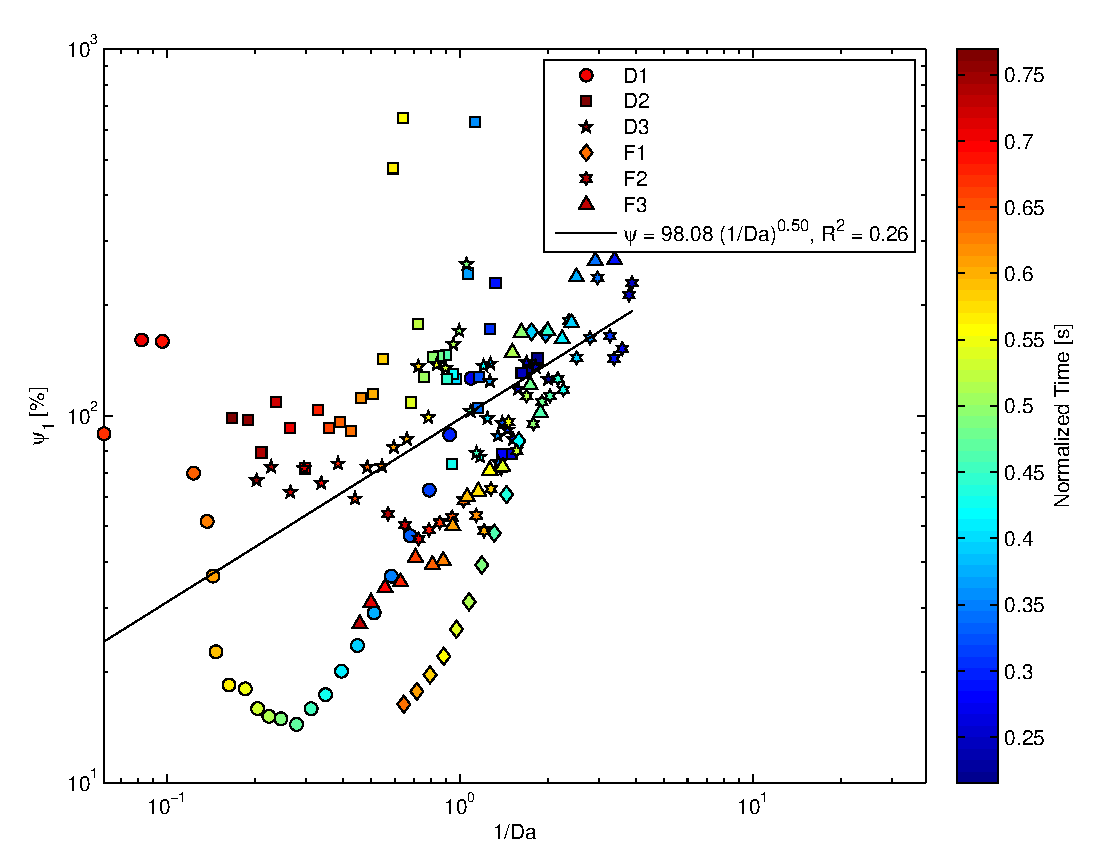
\includegraphics[width=0.45\linewidth]{Figures/phi1da}
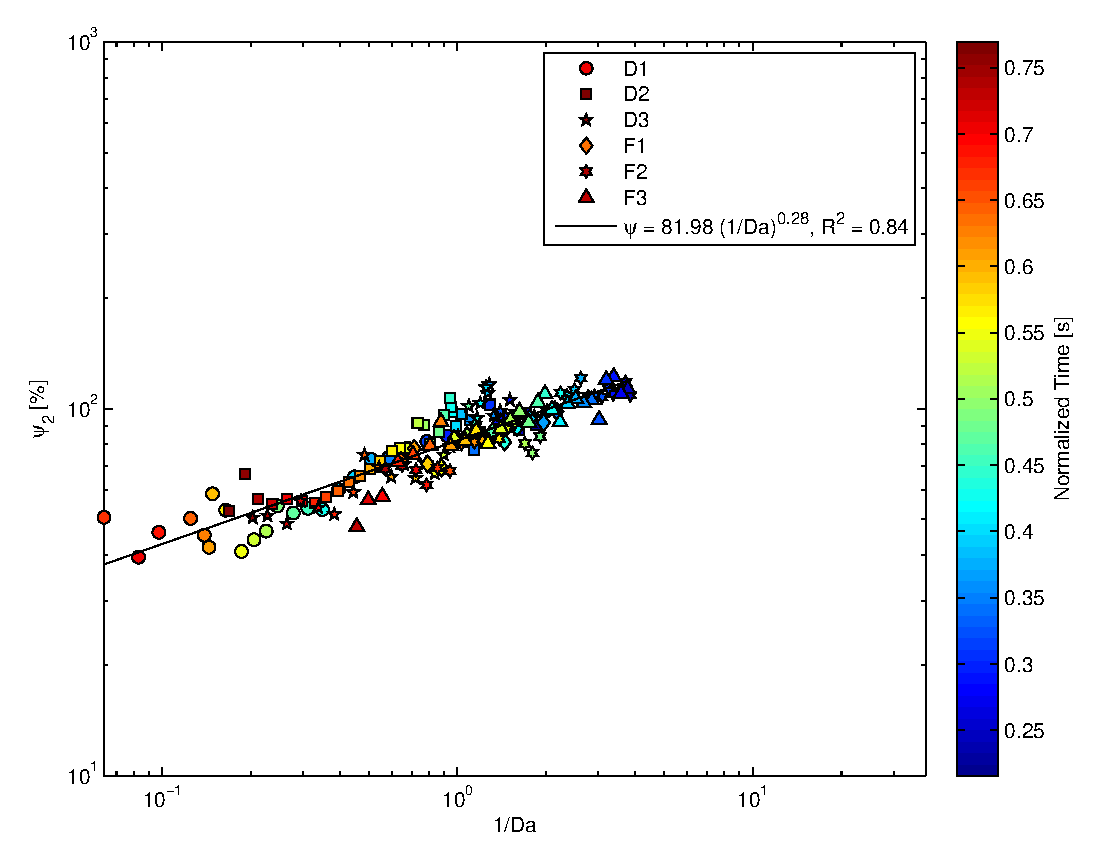
\includegraphics[width=0.45\linewidth]{Figures/phi2da}\\
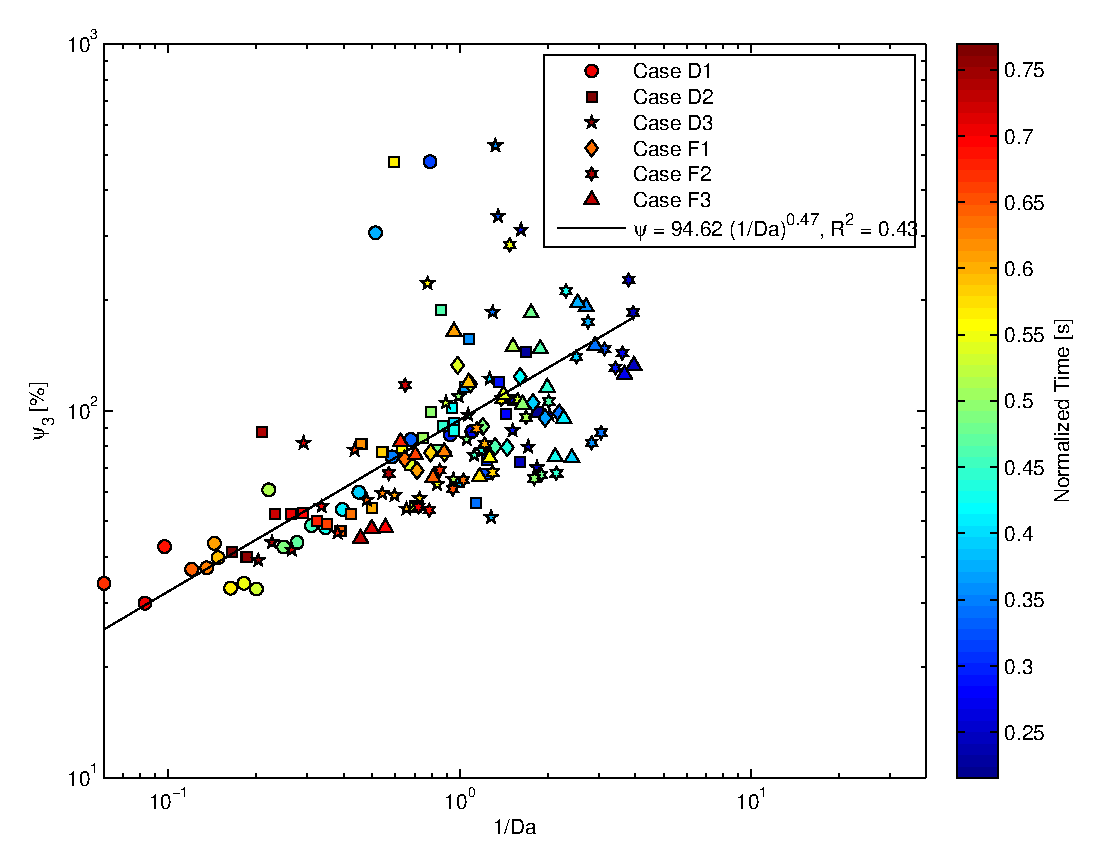
\includegraphics[width=0.45\linewidth]{Figures/phi3da}
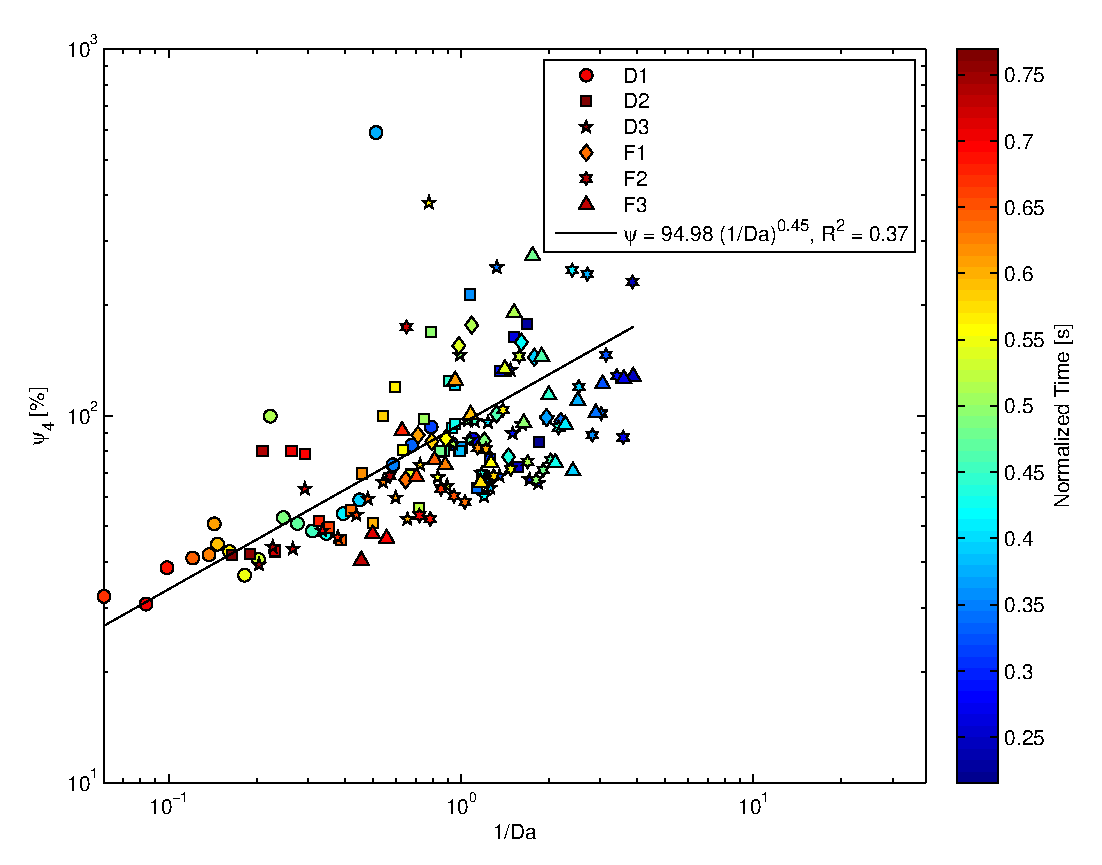
\includegraphics[width=0.45\linewidth]{Figures/phi4da}\\
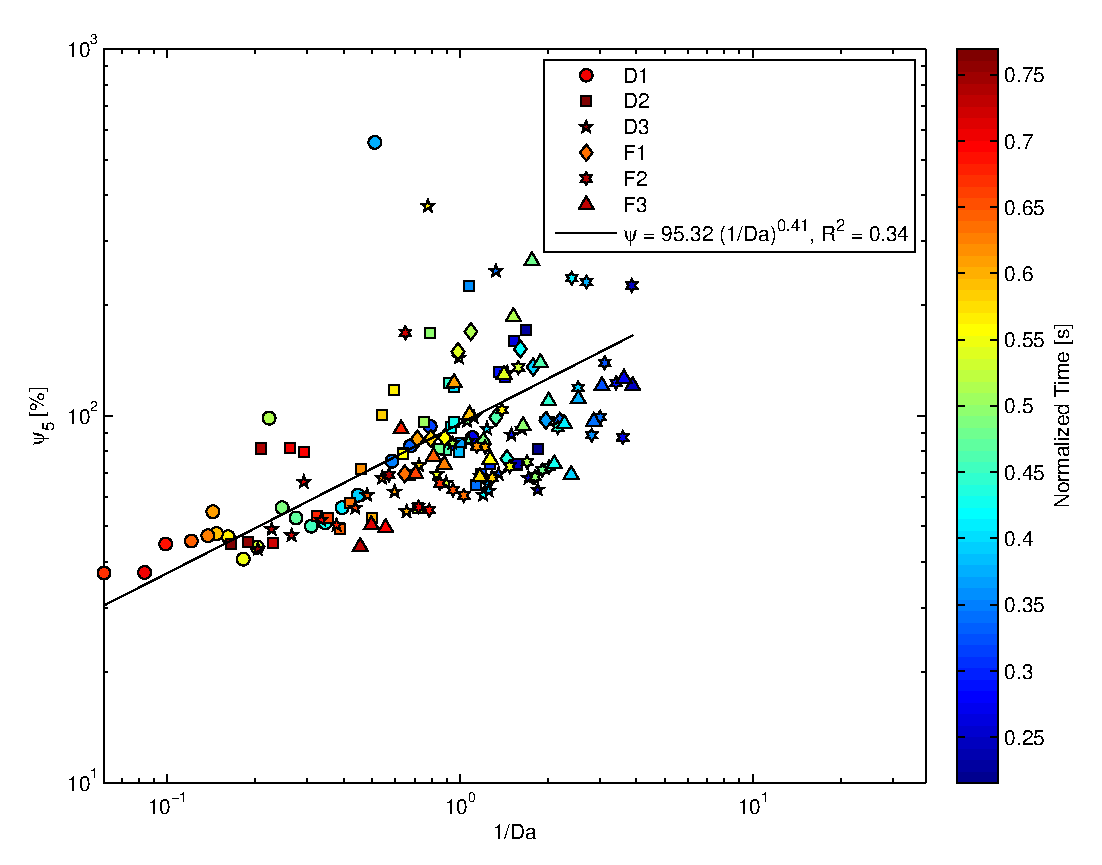
\includegraphics[width=0.45\linewidth]{Figures/phi5da}
\caption{Scatter plots of the five microphysical measures ($\psi_1$, $\psi_2$, $\psi_3$, $\psi_4$, $\psi_5$) of homogeneous mixing degree as a function of the inverse of the Damk\"ohler number ($Da$). Each point denotes the domain mean value for the corresponding scenario and time; the symbol and color the different simulation scenario and the normalized simulation time, respectively.\label{fig:PhiDa}}
\end{figure}

\begin{figure}[!htbp]\centering
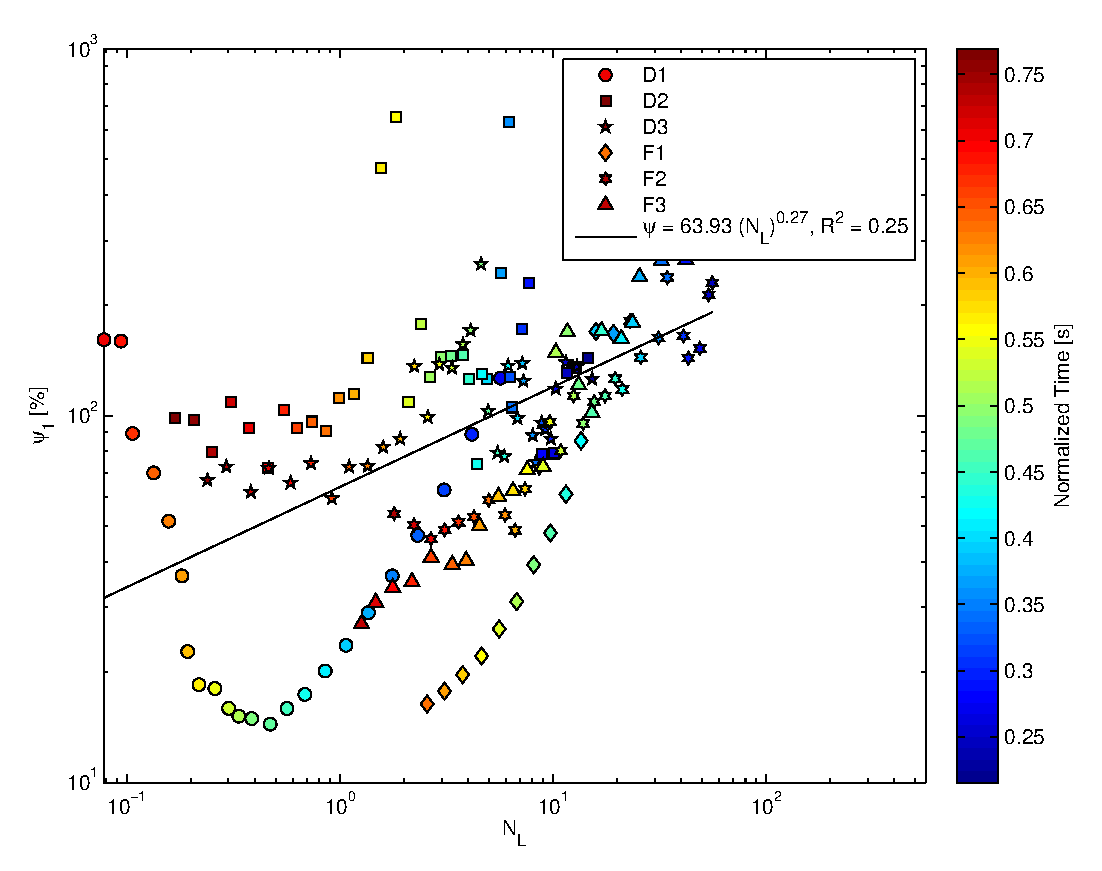
\includegraphics[width=0.45\linewidth]{Figures/phi1nl}
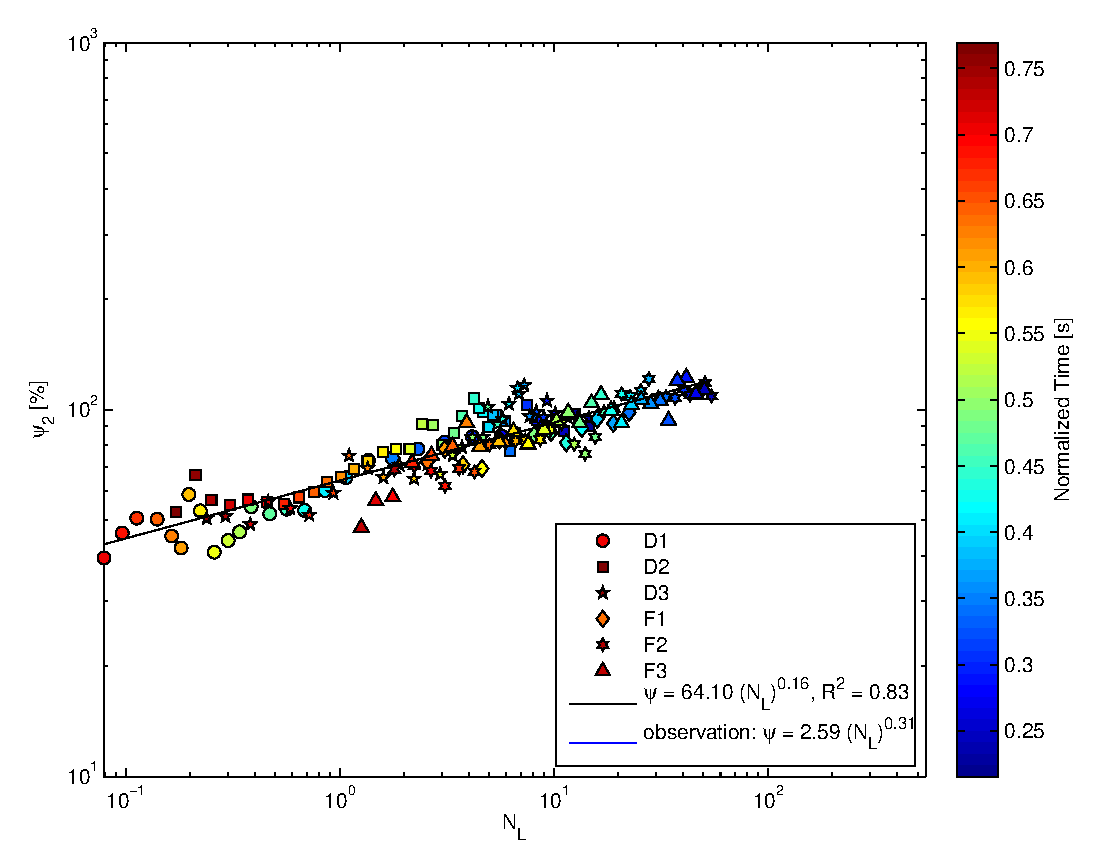
\includegraphics[width=0.45\linewidth]{Figures/phi2nl}\\
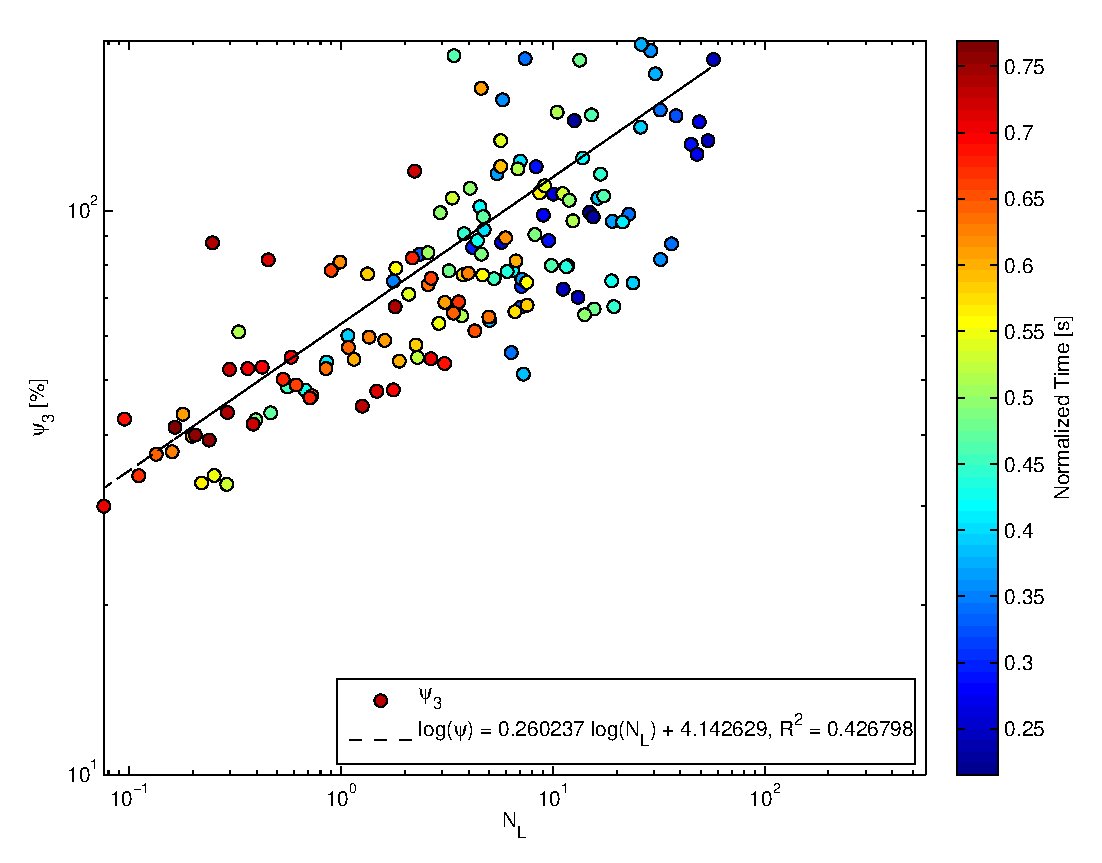
\includegraphics[width=0.45\linewidth]{Figures/phi3nl}
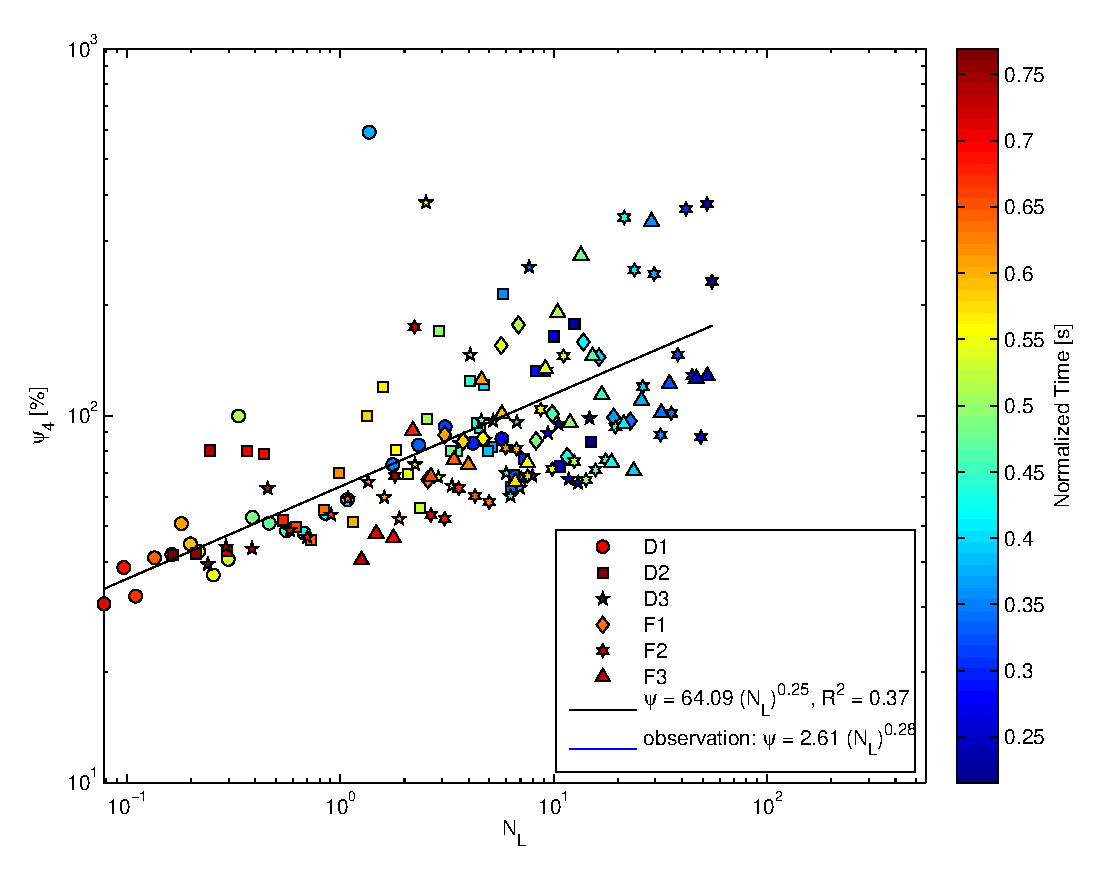
\includegraphics[width=0.45\linewidth]{Figures/phi4nl}\\
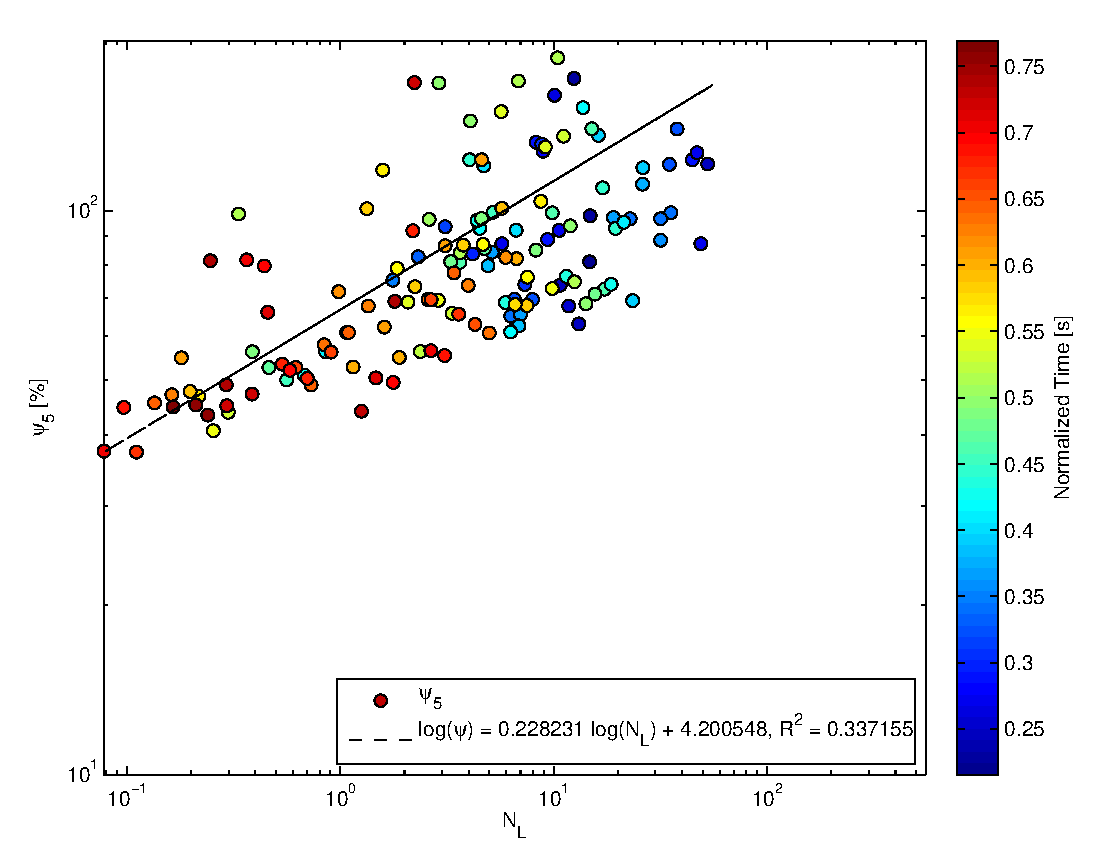
\includegraphics[width=0.45\linewidth]{Figures/phi5nl}
\caption{Scatter plots of the five microphysical measures of homogeneous mixing degree as a function of the transition scale number($N_L$). Each point denotes the domain mean value for the corresponding scenario and time; the symbol and color denote the different simulation scenario and the normalized simulation time, respectively.\label{fig:PhiNL}}
\end{figure}

Further inspection of the definitions of the Damk\"ohler number and transition scale number reveals that their essential difference lies in their use of different turbulent mixing length scales: the Damk\"ohler number is based on the Taylor length scale while the transition scale number is based on the transition scale. The close relationship between the two characteristic length scales \Fig{fig:TaylorScaleTranScale} confirms the virtually equivalent use of the two non-dimensional numbers in principle. However, the transition scale number is easier to estimate in practice, because the calculation of the Taylor length scale requires information on the spatial gradient of liquid water mixing ratio in addition to dissipation rate. Thus, all together, these results suggest that entrainment-mixing processes is best parameterized through $\psi_2$ as a function of transition scale number reinforcing the result of  \citep{Lu2013} based on observational analysis and EMPM simulations.     
\begin{figure}\centering
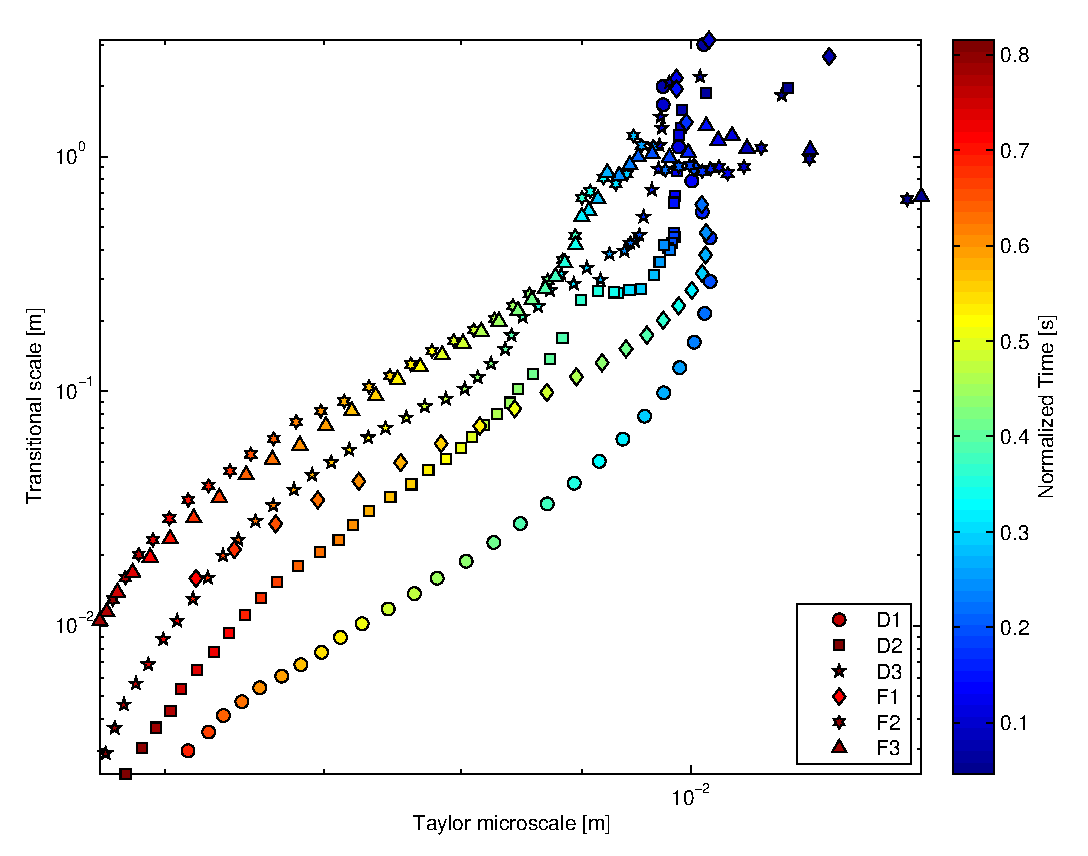
\includegraphics[width=0.5\linewidth]{Figures/taylor_trans}
\caption{Comparsion between the Taylor length scale and transition length scale. Each point denotes the domain mean value for the corresponding scenario and time. The symbol and color denotes the different simulations scenario and the normalized simulation time, respectively. \label{fig:TaylorScaleTranScale}}
\end{figure}

\section{Conclusions}\label{conclusion}
A new particle-resolved three dimensional direct numerical simulation (DNS) model is developed that combines the Lagrangian droplet tracking with the Eulerian field representation of turbulence near the Kolmogorov microscale. The new particle-resolved DNS uses the finite difference method coupled with WENO  scheme instead of the pseudo-spectral method on which most DNS models have been based on, thus providing more flexibility to deal with sharp cloud-air interfaces and non-periodic boundary conditions in future.

Six numerical experiments are performed to investigate the processes of entrainment of clear air and subsequent mixing with cloudy air and their interactions with cloud microphysics. The experiments are designed to represent different combinations of three initial cloudy areas (Case 1, 2 and 3), and two turbulence modes (decaying and forced turbulence). Case 1 corresponds to \citep{And04}, which aims to study the final stage of the mixing process. Case 2 tries to mimic the idealized cloud slab in \citep{Kumar12}. However, due to the Gibb's phenomena of the pseudo-spectral method, there is an inconsistency between the initial fields of cloud droplets and vapor mixing ratio in \citep{Kumar12}, in which an artificial continuous function was used to connect the area of cloudy air and clear air, while the cloud droplets were treated as a simple slab. This inconsistency is not desirable and is overcome here by taking advantage of the high resolution finite difference WENO scheme, which is designed for problems with piecewise smooth solutions containing discontinuities. Case 3 is created by rotating Case 2 with 90 degree clockwise to better mimic the cloud-top entrainment-mixing process and show the sedimentation effect on the entrainment-mixing processes and cloud droplet size distributions. All the simulation have been tested in modes of both decaying turbulence and forced turbulence. The thermodynamics and cloud microphysics are compared between different cases. The transient growth of turbulence kinetic energy due to buoyancy effects in the decaying cases agrees with the observation in \citep{Kumar14}. Analysis of the temporal changes of the droplet size distribution and key microphysical properties reveals that the initial configuration of cloudy areas effectively influence the mixing and microphysical processes in decaying turbulence. However, the effect of initial configuration seems to be much smaller in the forced turbulence. 

Five existing measures of microphysical homogeneous mixing degree are systematically examined, modified, and compared in terms of their ability as a unifying metric to represent the effect of various entrainment-mixing mechanisms on cloud microphysics. Also examined and compared are the conventional Damk\"{o}hler number and transition scale number as a dynamical measure of different mixing mechanisms. Further analysis of the relationship between the microphysical homogeneous mixing degree and the dynamical measure confirms the few previous studies \citep{And09,Lu2013,Lu2014} that despite the detailed differences among the six simulation scenarios in cloud properties, the variety of turbulent entrainment-mixing mechanisms can be reasonably represented with a power-law relationship between one of the microphysical homogeneous mixing degrees and one of the dynamical measures. The relationship between $\psi_2$ and transition scale number is recommended  for practical use. 

Two points are noteworthy. First, this study is focused on presenting the new particle-resolved DNS model and its general application to exploring the potential of developing a unified parameterization for effect of turbulent entrainment-mixing processes on cloud microphysics. The new model has other great potentials as well. For example, we plan to use the model to investigate the detailed effects of different factors such as turbulent intensity and environmental relative humidity. Another important topic to be examined is the interaction between turbulence and cloud microphysics, and the relative importance of turbulence and entrainment-mixing processes in shaping droplet size distributions. Second, similar to other DNS models, the domain DNS size used in this study is still too small to cover the full range of turbulent eddy sizes, which will require the model to run on high-performance supercomputing platform.  

\acknowledgments
The research was supported by the U.S. Department of Energy's Atmospheric System Research(ASR) and Earth System Modeling (ESM) programs and partially by the US Army Research Office under ARO-DURIP Grant W911NF-15-1-0403. Lu is supported by the National Natural Science Foundation of China and Jiangsu (91537108, BK20160041). The model results can be made available upon request.

%\bibliographystyle{agufull08}
%\bibliography{refs}
\begin{thebibliography}{60}
\providecommand{\natexlab}[1]{#1}
\expandafter\ifx\csname urlstyle\endcsname\relax
  \providecommand{\doi}[1]{doi:\discretionary{}{}{}#1}\else
  \providecommand{\doi}{doi:\discretionary{}{}{}\begingroup
  \urlstyle{rm}\Url}\fi

\bibitem[{\textit{Andrejczuk et~al.}(2004)\textit{Andrejczuk, Grabowski,
  Malinowski, and Smolarkiewicz}}]{And04}
Andrejczuk, M., W.-W. Grabowski, S.-P. Malinowski, and P.-K. Smolarkiewicz
  (2004), Numerical simulation of cloud-clear air interfacial mixing,
  \textit{Journal of the Atmospheric Sciences}, \textit{61}, 1726--1739.

\bibitem[{\textit{Andrejczuk et~al.}(2006)\textit{Andrejczuk, Grabowski,
  Malinowski, and Smolarkiewicz}}]{And06}
Andrejczuk, M., W.-W. Grabowski, S.-P. Malinowski, and P.-K. Smolarkiewicz
  (2006), Numerical simulation of cloud-clear air interfacial mixing: Effects
  on cloud microphysics, \textit{Journal of the Atmospheric Sciences},
  \textit{63}, 3204--3225.

\bibitem[{\textit{Andrejczuk et~al.}(2009)\textit{Andrejczuk, Grabowski,
  Malinowski, and Smolarkiewicz}}]{And09}
Andrejczuk, M., W.-W. Grabowski, S.-P. Malinowski, and P.-K. Smolarkiewicz
  (2009), Numerical simulation of cloud-clear air interfaical mixing:
  Homogeneous versus inhomogeneous mixing, \textit{Journal of the Atmospheric
  Sciences}, \textit{66}, 2493--2500.

\bibitem[{\textit{Baker et~al.}(1980)\textit{Baker, Corbin, and
  Latham}}]{Baker1980}
Baker, M., R.~Corbin, and J.~Latham (1980), The influence of entrainment on the
  evolution of cloud droplet spectra: I. a model of inhomogeneous mixing,
  \textit{Quarterly Journal of the Royal Meteorological Society},
  \textit{106}(449), 581--598.

\bibitem[{\textit{Balay et~al.}(2016)\textit{Balay, Abhyankar, Adams, Brown,
  Brune, Buschelman, Dalcin, Eijkhout, Kaushik, Knepley, McInnes, Rupp, Smith,
  Zampini, Zhang, and Zhang}}]{petsc_cite}
Balay, S., S.~Abhyankar, M.~F. Adams, J.~Brown, P.~Brune, K.~Buschelman,
  L.~Dalcin, V.~Eijkhout, W.~D. G.~D. Kaushik, M.~G. Knepley, L.~C. McInnes,
  K.~Rupp, B.~F. Smith, S.~Zampini, H.~Zhang, and H.~Zhang (2016), {PETS}c
  users manual, \textit{Tech. Rep. ANL-95/11 - Revision 3.7}, Argonne National
  Laboratory.

\bibitem[{\textit{Brenguier}(1993)}]{Brenguier1993}
Brenguier, J.-L. (1993), Observations of cloud microstructure at the centimeter
  scale, \textit{Journal of Applied Meteorology}, \textit{32}(4), 783--793.

\bibitem[{\textit{Brown et~al.}(2001)\textit{Brown, Cortez, and
  Minion}}]{Brown2001}
Brown, D.~L., R.~Cortez, and M.~L. Minion (2001), Accurate projection methods
  for the incompressible navier{\textendash}stokes equations, \textit{Journal
  of Computational Physics}, \textit{168}(2), 464--499,
  \doi{10.1006/jcph.2001.6715}.

\bibitem[{\textit{Burnet and Brenguier}(2007)}]{Burnet2007Observational}
Burnet, F., and J.-L. Brenguier (2007), Observational study of the
  entrainment-mixing process in warm convective clouds, \textit{Journal of the
  Atmospheric Sciences}, \textit{64}(6), 1995--2011, \doi{10.1175/jas3928.1}.

\bibitem[{\textit{Burnet et~al.}(1992)\textit{Burnet, Wurm, Yarnold, Peacock,
  Nyman, and Turesson}}]{Burnet1992}
Burnet, N., R.~Wurm, J.~Yarnold, J.~Peacock, J.~Nyman, and I.~Turesson (1992),
  Prediction of normal-tissue tolerance to radiotherapy from in-vitro cellular
  radiation sensitivity, \textit{The Lancet}, \textit{339}(8809), 1570--1571.

\bibitem[{\textit{Celani et~al.}(2005)\textit{Celani, Falkovich, Mazzino, and
  Seminara}}]{Celani05}
Celani, A., G.~Falkovich, A.~Mazzino, and Seminara (2005), Droplet condensation
  in turbulence flows, \textit{Europhysics Letters}, \textit{70}(6), 775--781.

\bibitem[{\textit{Chosson et~al.}(2007)\textit{Chosson, Brenguier, and
  Sch{\"u}ller}}]{Chosson2007}
Chosson, F., J.-L. Brenguier, and L.~Sch{\"u}ller (2007), Entrainment-mixing
  and radiative transfer simulation in boundary layer clouds, \textit{Journal
  of the atmospheric sciences}, \textit{64}(7), 2670--2682.

\bibitem[{\textit{de~Lozar and Mellado}(2013)}]{LozarMellado2013}
de~Lozar, A., and J.~P. Mellado (2013), Direct numerical simulations of a smoke
  cloud--top mixing layer as a model for stratocumuli, \textit{Journal of the
  Atmospheric Sciences}, \textit{70}(8), 2356--2375.

\bibitem[{\textit{Devenish et~al.}(2012)\textit{Devenish, Bartello, Brenguier,
  Collins, Grabowski, IJzermans, Malinowski, Reeks, Vassilicos, Wang
  et~al.}}]{Devenish2012}
Devenish, B., P.~Bartello, J.-L. Brenguier, L.~Collins, W.~Grabowski,
  R.~IJzermans, S.~Malinowski, M.~Reeks, J.~Vassilicos, L.-P. Wang, et~al.
  (2012), Droplet growth in warm turbulent clouds, \textit{Quarterly Journal of
  the Royal Meteorological Society}, \textit{138}(667), 1401--1429.

\bibitem[{\textit{Eaton and Fessler}(1994)}]{Eaton94}
Eaton, J.~K., and J.~R. Fessler (1994), Preferential concentration of particles
  by turbulence, \textit{International Journal of Multiphase Flow},
  \textit{20}(Supplement 1), 169--209.

\bibitem[{\textit{Endo et~al.}(2015)\textit{Endo, Fridlind, Lin, Vogelmann,
  Toto, Ackerman, McFarquhar, Jackson, Jonsson, and Liu}}]{Endo2015}
Endo, S., A.~M. Fridlind, W.~Lin, A.~M. Vogelmann, T.~Toto, A.~S. Ackerman,
  G.~M. McFarquhar, R.~C. Jackson, H.~H. Jonsson, and Y.~Liu (2015), Racoro
  continental boundary layer cloud investigations: 2. large-eddy simulations of
  cumulus clouds and evaluation with in situ and ground-based observations,
  \textit{Journal of Geophysical Research: Atmospheres}, \textit{120}(12),
  5993--6014.

\bibitem[{\textit{Falgout and Yang}(2002)}]{hypre_cite}
Falgout, R.~D., and U.~M. Yang (2002), hypre: A library of high performance
  preconditioners, in \textit{Lecture Notes in Computer Science}, pp. 632--641,
  Springer Science and Business Media.

\bibitem[{\textit{Ghosal et~al.}(1995)\textit{Ghosal, Lund, Moin, and
  Akselvoll}}]{ghosal1995dynamic}
Ghosal, S., T.~S. Lund, P.~Moin, and K.~Akselvoll (1995), A dynamic
  localization model for large-eddy simulation of turbulent flows,
  \textit{Journal of Fluid Mechanics}, \textit{286}, 229--255.

\bibitem[{\textit{Grabowski et~al.}(2006)\textit{Grabowski, Bechtold, Cheng,
  Forbes, Halliwell, Khairoutdinov, Lang, Nasuno, Petch, Tao
  et~al.}}]{Grabowski2006}
Grabowski, W., P.~Bechtold, A.~Cheng, R.~Forbes, C.~Halliwell,
  M.~Khairoutdinov, S.~Lang, T.~Nasuno, J.~Petch, W.-K. Tao, et~al. (2006),
  Daytime convective development over land: A model intercomparison based on
  lba observations, \textit{Quarterly Journal of the Royal Meteorological
  Society}, \textit{132}(615), 317--344.

\bibitem[{\textit{Grabowski}(1993)}]{Grabowski1993Cumulus}
Grabowski, W.~W. (1993), Cumulus entrainment, fine-scale mixing, and buoyancy
  reversal, \textit{Quarterly Journal of the Royal Meteorological Society},
  \textit{119}(513), 935--956, \doi{10.1002/qj.49711951305}.

\bibitem[{\textit{Grabowski and Wang}(2013)}]{GrabowskiWang2013}
Grabowski, W.~W., and L.-P. Wang (2013), Growth of cloud droplets in a
  turbulent environment, \textit{Annual Review of Fluid Mechanics},
  \textit{45}, 293--324.

\bibitem[{\textit{Hicks et~al.}(1990)\textit{Hicks, Pontikis, and
  Rigaud}}]{Hicks1990}
Hicks, E., C.~Pontikis, and A.~Rigaud (1990), Entrainment and mixing processes
  as related to droplet growth in warm midlatitude and tropical clouds,
  \textit{Journal of the atmospheric sciences}, \textit{47}(13), 1589--1618.

\bibitem[{\textit{Howell}(1949)}]{Howell1949}
Howell, W.~E. (1949), The growth of cloud drops in uniformly cooled air,
  \textit{Journal of Meteorology}, \textit{6}(2), 134--149.

\bibitem[{\textit{Hsiu-chi}(1964)}]{Zhou1964}
Hsiu-chi, C. (1964), A study of the microphysical mechanism of warm-cloud
  precipitation, \textit{Tech. rep.}, DTIC Document.

\bibitem[{\textit{Hudson and Yum}(1997)}]{HudsonYum1997}
Hudson, J.~G., and S.~S. Yum (1997), Droplet spectral broadening in marine
  stratus, \textit{Journal of the atmospheric sciences}, \textit{54}(22),
  2642--2654.

\bibitem[{\textit{Jiang and Shu}(1996)}]{JiangShu1996}
Jiang, G.-S., and C.-W. Shu (1996), Efficient implementation of weighted eno
  schemes, \textit{Journal of computational physics}, \textit{126}(1),
  202--228.

\bibitem[{\textit{Khvorostyanov and Curry}(1999)}]{KhvorostyanovCurry1999}
Khvorostyanov, V.~I., and J.~A. Curry (1999), Toward the theory of stochastic
  condensation in clouds. part i: A general kinetic equation, \textit{Journal
  of the atmospheric sciences}, \textit{56}(23), 3985--3996.

\bibitem[{\textit{Krueger et~al.}(1997)\textit{Krueger, Su, and
  McMurtry}}]{Krueger1997Modeling}
Krueger, S.~K., C.-W. Su, and P.~A. McMurtry (1997), Modeling entrainment and
  finescale mixing in cumulus clouds, \textit{Journal of the atmospheric
  sciences}, \textit{54}(23), 2697--2712.

\bibitem[{\textit{Kumar et~al.}(2012{\natexlab{a}})\textit{Kumar, Schumacher,
  and R.-A.Shaw}}]{Kumar11}
Kumar, B., J.~Schumacher, and R.-A.Shaw (2012{\natexlab{a}}), Cloud
  microphysical effects of turbulent mixing and entrainment,
  \textit{Theoretical Computational Fluid Dynamics}, \textit{27}(361).

\bibitem[{\textit{Kumar et~al.}(2012{\natexlab{b}})\textit{Kumar, Janetzko,
  Schumacher, and R.-A.Shaw}}]{Kumar12}
Kumar, B., F.~Janetzko, J.~Schumacher, and R.-A.Shaw (2012{\natexlab{b}}),
  Extreme response of a coupled scalar-particle system during turbulent mixing,
  \textit{New Journal of Physics}, \textit{14}(115020).

\bibitem[{\textit{Kumar et~al.}(2014)\textit{Kumar, Schumacher, and
  R.-A.Shaw}}]{Kumar14}
Kumar, B., J.~Schumacher, and R.-A.Shaw (2014), Lagrangian mixing dynamics at
  the cloudy-clear air interface, \textit{Journal of the Atmospheric Sciences},
  \textit{71}(7), 2564--2580.

\bibitem[{\textit{Lanotte et~al.}(2009)\textit{Lanotte, Seminara, and
  Toschi}}]{Lanotte2009}
Lanotte, A.~S., A.~Seminara, and F.~Toschi (2009), Cloud droplet growth by
  condensation in homogeneous isotropic turbulence, \textit{J. Atmos. Sci.},
  \textit{66}(6), 1685--1697, \doi{10.1175/2008jas2864.1}.

\bibitem[{\textit{Lehmann et~al.}(2009{\natexlab{a}})\textit{Lehmann, Siebert,
  and R.-A.Shaw}}]{Lehmann09}
Lehmann, K., H.~Siebert, and R.-A.Shaw (2009{\natexlab{a}}), Homogeneous and
  inhomogeneous mixing in cumulus clouds: Dependence on local turbulence
  structure, \textit{Journal of the Atmospheric Sciences}, \textit{66},
  3641--3659.

\bibitem[{\textit{Lehmann et~al.}(2009{\natexlab{b}})\textit{Lehmann, Siebert,
  and Shaw}}]{Lehmann2009}
Lehmann, K., H.~Siebert, and R.~A. Shaw (2009{\natexlab{b}}), Homogeneous and
  inhomogeneous mixing in cumulus clouds: Dependence on local turbulence
  structure, \textit{Journal of the Atmospheric Sciences}, \textit{66}(12),
  3641--3659, \doi{10.1175/2009jas3012.1}.

\bibitem[{\textit{Liu and Daum}(2002)}]{Liu2002}
Liu, Y., and P.~H. Daum (2002), Anthropogenic aerosols: Indirect warming effect
  from dispersion forcing, \textit{Nature}, \textit{419}(6907), 580.

\bibitem[{\textit{Liu and Hallett}(1997)}]{LiuHallett1997}
Liu, Y., and J.~Hallett (1997), The ‘1/3’power law between effective radius
  and liquid-water content, \textit{Quarterly Journal of the Royal
  Meteorological Society}, \textit{123}(542), 1789--1795.

\bibitem[{\textit{Liu and Hallett}(1998)}]{LiuHallett1998}
Liu, Y., and J.~Hallett (1998), On size distributions of cloud droplets growing
  by condensation: A new conceptual model, \textit{Journal of the atmospheric
  sciences}, \textit{55}(4), 527--536.

\bibitem[{\textit{Liu et~al.}(1995)\textit{Liu, Laiguang, Weinong, and
  Feng}}]{Liu1995}
Liu, Y., Y.~Laiguang, Y.~Weinong, and L.~Feng (1995), On the size distribution
  of cloud droplets, \textit{Atmospheric Research}, \textit{35}(2), 201--216.

\bibitem[{\textit{Liu et~al.}(2004)\textit{Liu, Daum, and
  McGraw}}]{MacGrawLiu2004}
Liu, Y., P.~H. Daum, and R.~McGraw (2004), An analytical expression for
  predicting the critical radius in the autoconversion parameterization,
  \textit{Geophysical research letters}, \textit{31}(6).

\bibitem[{\textit{Lu et~al.}(2011)\textit{Lu, Liu, and Niu}}]{Lu2011}
Lu, C., Y.~Liu, and S.~Niu (2011), Examination of turbulent entrainment-mixing
  mechanisms using a combined approach, \textit{J. Geophys. Res.},
  \textit{116}(D20), \doi{10.1029/2011jd015944}.

\bibitem[{\textit{Lu et~al.}(2013)\textit{Lu, Liu, Niu, Krueger, and
  Wagner}}]{Lu2013}
Lu, C., Y.~Liu, S.~Niu, S.~Krueger, and T.~Wagner (2013), Exploring
  parameterization for turbulent entrainment-mixing processes in clouds,
  \textit{Journal of Geophysical Research: Atmospheres}, \textit{118}(1),
  185--194, \doi{10.1029/2012jd018464}.

\bibitem[{\textit{Lu et~al.}(2014)\textit{Lu, Liu, Niu, and Endo}}]{Lu2014}
Lu, C., Y.~Liu, S.~Niu, and S.~Endo (2014), Scale dependence of
  entrainment-mixing mechanisms in cumulus clouds, \textit{Journal of
  Geophysical Research: Atmospheres}, \textit{119}(24).

\bibitem[{\textit{Malinowski et~al.}(2008)\textit{Malinowski, Andrejczuk,
  Grabowski, Korczyk, Kowalewski, and Smolarkiewicz}}]{Malinowski2008}
Malinowski, S.~P., M.~Andrejczuk, W.~W. Grabowski, P.~Korczyk, T.~A.
  Kowalewski, and P.~K. Smolarkiewicz (2008), Laboratory and modeling studies
  of cloud{\textendash}clear air interfacial mixing: anisotropy of small-scale
  turbulence due to evaporative cooling, \textit{New Journal of Physics},
  \textit{10}(7), 075,020, \doi{10.1088/1367-2630/10/7/075020}.

\bibitem[{\textit{McGraw and Liu}(2003)}]{McGrawLiu2003}
McGraw, R., and Y.~Liu (2003), Kinetic potential and barrier crossing: A model
  for warm cloud drizzle formation, \textit{Physical review letters},
  \textit{90}(1), 018,501.

\bibitem[{\textit{McGraw and Liu}(2006)}]{MacGrawLiu2006}
McGraw, R., and Y.~Liu (2006), Brownian drift-diffusion model for evolution of
  droplet size distributions in turbulent clouds, \textit{Geophysical research
  letters}, \textit{33}(3).

\bibitem[{\textit{Orszag}(1972)}]{Orszag72}
Orszag, S.~A. (1972), Comparison of pseudospectral and spectral approximation,
  \textit{Studies in Applied Mathematics}, \textit{51}(3), 253--259,
  \doi{10.1002/sapm1972513253}.

\bibitem[{\textit{Rogallo}(1981)}]{Rogallo81}
Rogallo, R.~S. (1981), \textit{Numerical Experiments in Homogeneous
  Turbulence}, vol. 81315, National Aeronautics and Space Administration.

\bibitem[{\textit{Rosales and Meneveau}(2005)}]{Rosales05}
Rosales, C., and C.~Meneveau (2005), Linear forcing in numerical simulations of
  isotropic turbulence: Physical space implementations and convergence
  properties, \textit{Physics of Fluids}, \textit{17}(9), 095,106.

\bibitem[{\textit{Sedunov}(1974)}]{Sedunov1974}
Sedunov, Y.~S. (1974), \textit{Physics of Drop Formation in the Atmosphere},
  Wiley-Blackwell.

\bibitem[{\textit{Shaw et~al.}(1998)\textit{Shaw, Reade, Collins, and
  Verlinde}}]{Shaw1998}
Shaw, R.~A., W.~C. Reade, L.~R. Collins, and J.~Verlinde (1998), Preferential
  concentration of cloud droplets by turbulence: Effects on the early evolution
  of cumulus cloud droplet spectra, \textit{Journal of the atmospheric
  sciences}, \textit{55}(11), 1965--1976.

\bibitem[{\textit{Slawinska et~al.}(2008)\textit{Slawinska, Grabowski,
  Pawlowska, and Wyszogrodzki}}]{Slawinska2008}
Slawinska, J., W.~W. Grabowski, H.~Pawlowska, and A.~A. Wyszogrodzki (2008),
  Optical properties of shallow convective clouds diagnosed from a
  bulk-microphysics large-eddy simulation, \textit{Journal of Climate},
  \textit{21}(7), 1639--1647.

\bibitem[{\textit{Su et~al.}(1998)\textit{Su, Krueger, McMurtry, and
  Austin}}]{Su1998}
Su, C.-W., S.~K. Krueger, P.~A. McMurtry, and P.~H. Austin (1998), Linear eddy
  modeling of droplet spectral evolution during entrainment and mixing in
  cumulus clouds, \textit{Atmospheric research}, \textit{47}, 41--58.

\bibitem[{\textit{Sullivan et~al.}(1994)\textit{Sullivan, McWilliams, and
  Moeng}}]{Sullivan1994}
Sullivan, P.~P., J.~C. McWilliams, and C.-H. Moeng (1994), A subgrid-scale
  model for large-eddy simulation of planetary boundary-layer flows,
  \textit{Boundary-Layer Meteorology}, \textit{71}(3), 247--276.

\bibitem[{\textit{Telford and Chai}(1980)}]{TelfordChai1980}
Telford, J.~W., and S.~K. Chai (1980), A new aspect of condensation theory,
  \textit{pure and applied geophysics}, \textit{118}(2), 720--742.

\bibitem[{\textit{Vaillancourt and Yau}(2000)}]{Vaillancourt00}
Vaillancourt, P.~A., and M.~K. Yau (2000), Review of particle-turbulence
  interactions and consequences for cloud physics, \textit{American
  Meteorological Society}, \textit{81}(2), 285--298.

\bibitem[{\textit{Vaillancourt et~al.}(2002)\textit{Vaillancourt, Yau,
  Bartello, and Grabowski}}]{Vaillancourt02}
Vaillancourt, P.~A., M.~K. Yau, P.~Bartello, and W.~W. Grabowski (2002),
  Microscopic approach to cloud droplets growth by condensation. part ii:
  Turbulence, clustering, and condensational growth, \textit{American
  Meteorological Society}, \textit{59}, 3421--3432.

\bibitem[{\textit{Warner}(1973)}]{Warner1973}
Warner, J. (1973), The microstructure of cumulus cloud: Part iv. the effect on
  the droplet spectrum of mixing between cloud and environment, \textit{Journal
  of the Atmospheric Sciences}, \textit{30}(2), 256--261.

\bibitem[{\textit{Yano and Moncrieff}(2016)}]{Yano2016}
Yano, J.-I., and M.~W. Moncrieff (2016), Numerical archetypal parameterization
  for mesoscale convective systems, \textit{Journal of the Atmospheric
  Sciences}, \textit{73}(7), 2585--2602.

\bibitem[{\textit{Yau and Rogers}(1996)}]{RogersYau1996}
Yau, M.~K., and R.~Rogers (1996), \textit{A short course in cloud physics},
  Elsevier.

\bibitem[{\textit{Yum and Hudson}(2005)}]{YumHudson2005}
Yum, S.~S., and J.~G. Hudson (2005), Adiabatic predictions and observations of
  cloud droplet spectral broadness, \textit{Atmospheric research},
  \textit{73}(3), 203--223.

\bibitem[{\textit{Yum et~al.}(2015)\textit{Yum, Wang, Liu, Senum, Springston,
  McGraw, and Yeom}}]{Yum2015}
Yum, S.~S., J.~Wang, Y.~Liu, G.~Senum, S.~Springston, R.~McGraw, and J.~M. Yeom
  (2015), Cloud microphysical relationships and their implication on
  entrainment and mixing mechanism for the stratocumulus clouds measured during
  the vocals project, \textit{Journal of Geophysical Research: Atmospheres},
  \textit{120}(10), 5047--5069.

\end{thebibliography}

\newpage
\section*{Figure captions}
\begin{enumerate}[label=Figure \arabic*:\,, leftmargin=0cm,itemindent=.5cm,labelwidth=\itemindent,labelsep=0cm,align=left]
\item \nameref{fig:eng_spr}

\item \nameref{fig:slice_case123}

\item \nameref{fig:therm_dynam}

\item \nameref{fig:rad_distri}

\item \nameref{fig:temporal_variation}

\item \nameref{fig:mixing_diagram}

\item \nameref{phi_compare}

\item \nameref{fig:PhiDa}

\item \nameref{fig:PhiNL}

\item \nameref{fig:TaylorScaleTranScale}


\end{enumerate}

\end{document}
